\documentclass[aps,rmp,preprint,superscriptaddress,10pt,onecolumn]{article}
\usepackage[utf8x]{inputenc}
\usepackage{amsmath,amsthm,amsfonts,amssymb,amscd}
\usepackage{graphicx}
\usepackage{wrapfig}
\usepackage{enumerate}
\usepackage{color}
\usepackage[final]{hyperref}
\usepackage{fontspec}
%\usepackage{natbib}
%\bibliographystyle{plainnat}


\setmainfont{Times New Roman}
\usepackage{unicode-math}
\setmathfont{XITS Math}


%\setlength{\parindent}{20pt}
\def\thesubsectiondis{\unskip\arabic{subsection}}
 
\begin{document}

\title{Data summary:\\\textit{Growth: From Microorganisms to Megacities}, Vaclav Smil (2009)}
\author{Liam P. Shaw}
\date{\today}


\maketitle

\section*{Summary}

\noindent This document contains graphs fitted from a variety of datasets in \textit{Growth} (Smil, 2009). Code and data to reproduce analysis are available at \url{https://github.com/liampshaw/Smil-Growth-2009}. 
\begin{figure}[h]
\includegraphics[width=8cm]{output/figs-ggplot/1.6.pdf}
\caption{\textbf{Dataset 1.6}: "Prediction of growth of US air travel (in billions of passenger-kilometers) based on the period 1930-1980 (top}
\end{figure}
	
\begin{figure}[h]
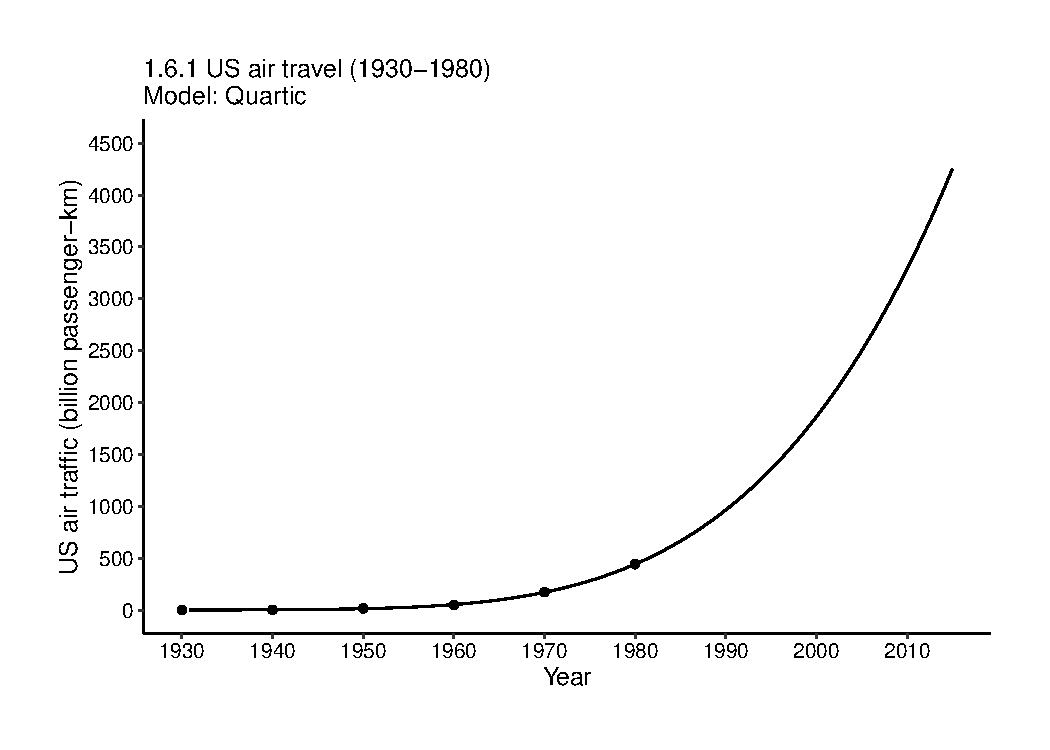
\includegraphics[width=8cm]{output/figs-ggplot/1.6.1.pdf}
\caption{\textbf{Dataset 1.6.1}: Prediction of growth of US air travel (in billions of passenger-kilometers) based on the period 1930-1980. The best fit is a quartic regression. Data from various annual reports by the International Civil Aviation Organization. }
\end{figure}
	
\begin{figure}[h]
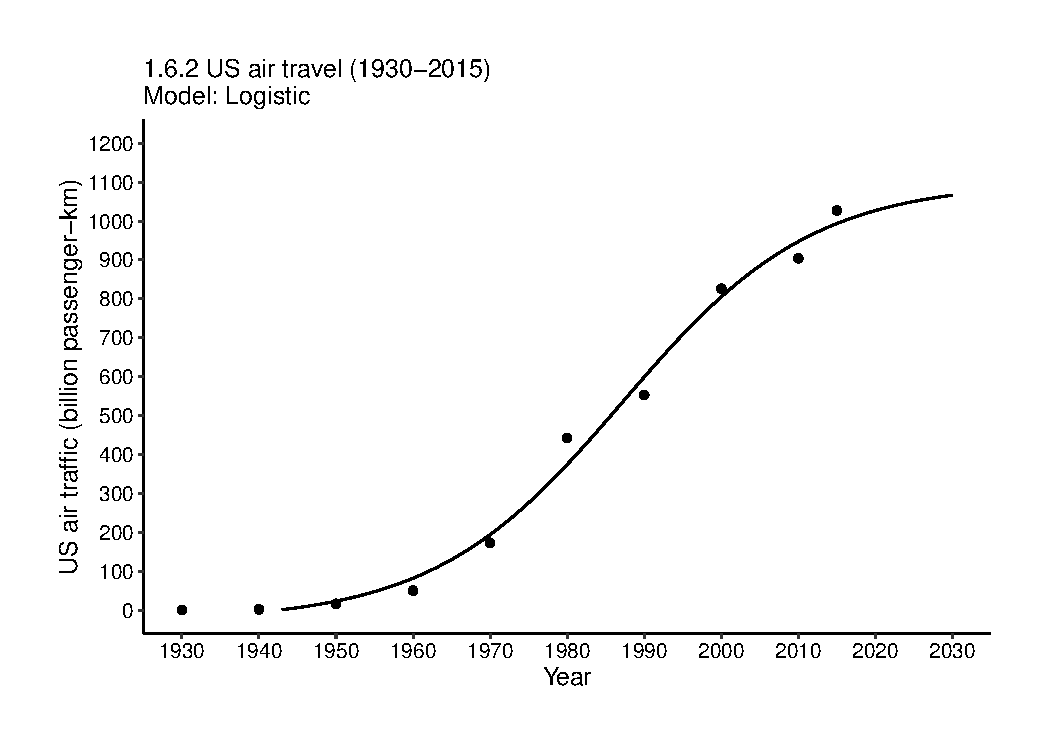
\includegraphics[width=8cm]{output/figs-ggplot/1.6.2.pdf}
\caption{\textbf{Dataset 1.6.2}: Prediction of growth of US air travel (in billions of passenger-kilometers) based on the period 1930-2015. The best fit is a logistic curve with the inflection year in 1987. Data from various annual reports by the International Civil Aviation Organization. }
\end{figure}
	
\begin{figure}[h]
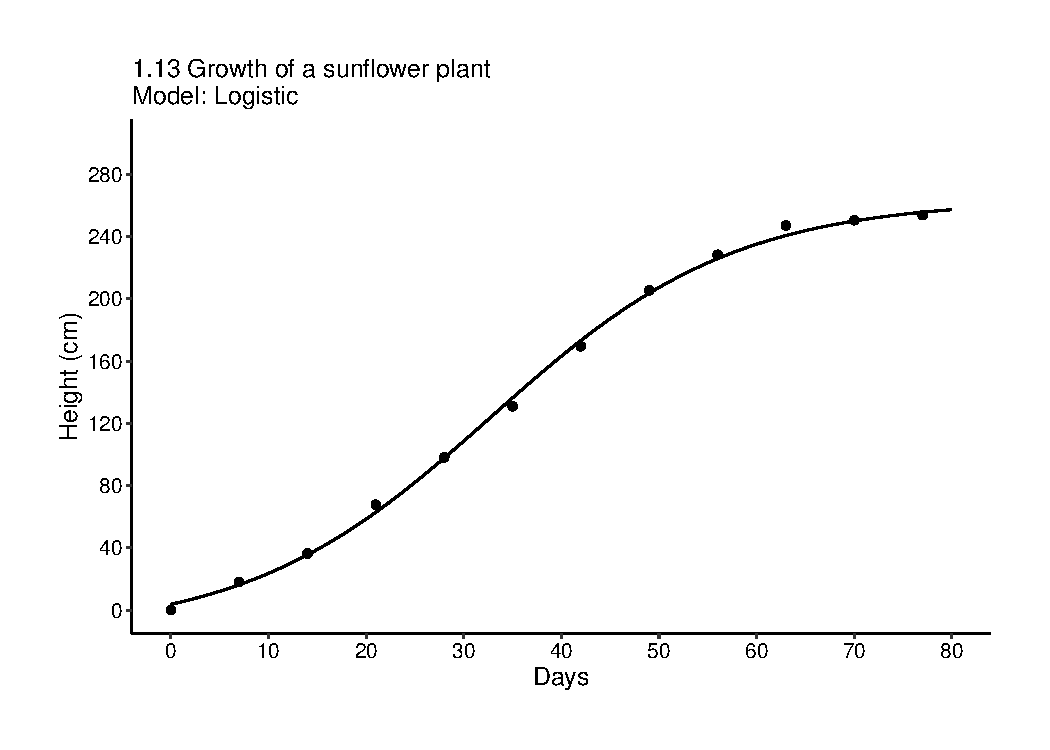
\includegraphics[width=8cm]{output/figs-ggplot/1.13.pdf}
\caption{\textbf{Dataset 1.13}: "Logistic growth (inflection point at 37.1 days}
\end{figure}
	
\begin{figure}[h]
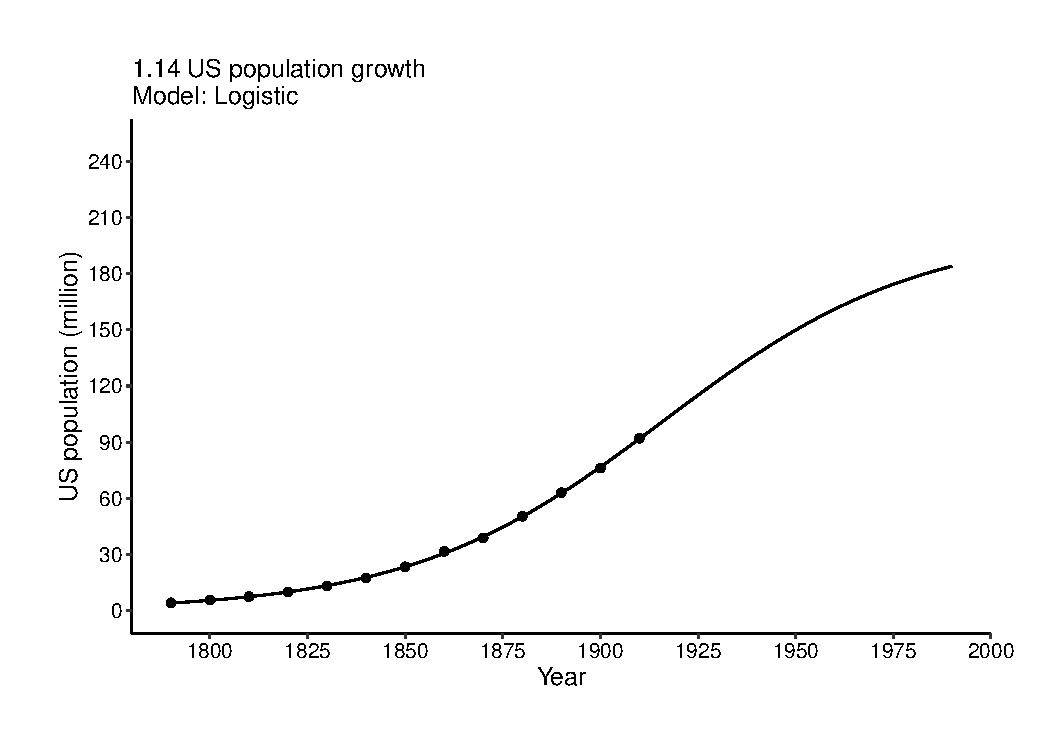
\includegraphics[width=8cm]{output/figs-ggplot/1.14.pdf}
\caption{\textbf{Dataset 1.14}: "Forecast of US population growth based on the logistic curve (inflection point in 1919}
\end{figure}
	
\begin{figure}[h]
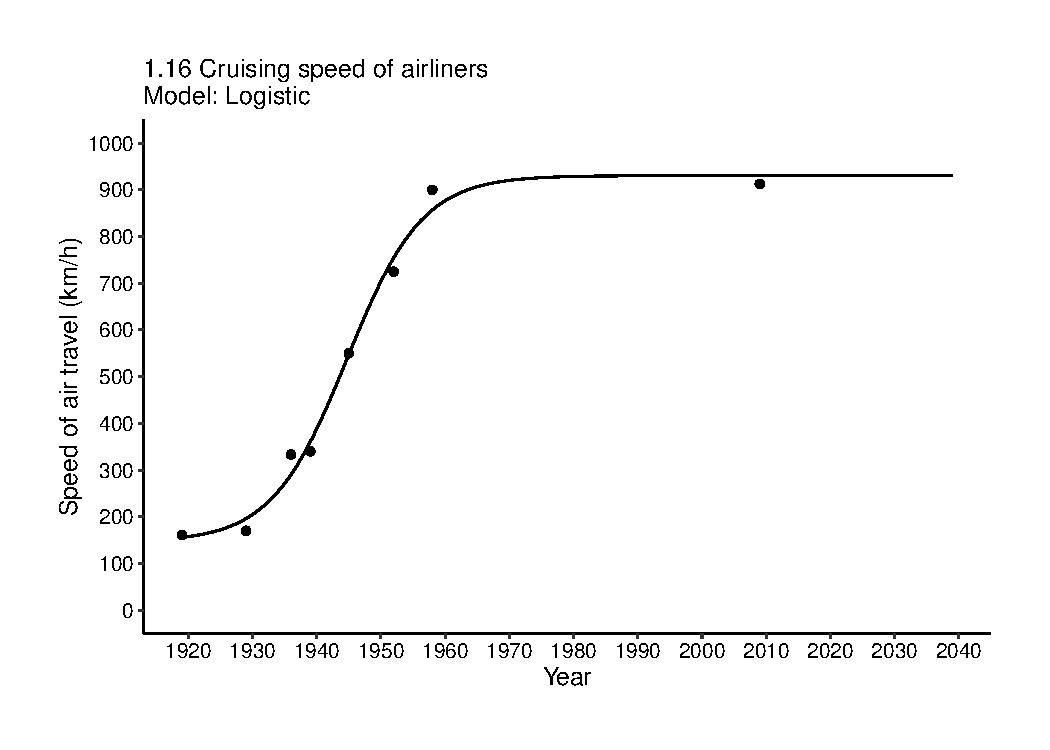
\includegraphics[width=8cm]{output/figs-ggplot/1.16.pdf}
\caption{\textbf{Dataset 1.16}: "Logistic curve tracing the growth of cruising speed of commercial airliners 1919-2039 (inflection point in 1945}
\end{figure}
	
\begin{figure}[h]
\includegraphics[width=8cm]{output/figs-ggplot/1.17.pdf}
\caption{\textbf{Dataset 1.17}: Fitting Mozart's oeuvre into growth curves: symmetrical (a)and asymmetrical (b) logistic functions and quadratic (c) and quartic (d) regression all have high degrees of fit (R^2=0.99) but predict substantially different long-term outcomes for the year 1806 when Mozart (who died in 1791) would have been 50 years old. Compositions by date listed in Giegling et al. (1964).}
\end{figure}
	
\begin{figure}[h]
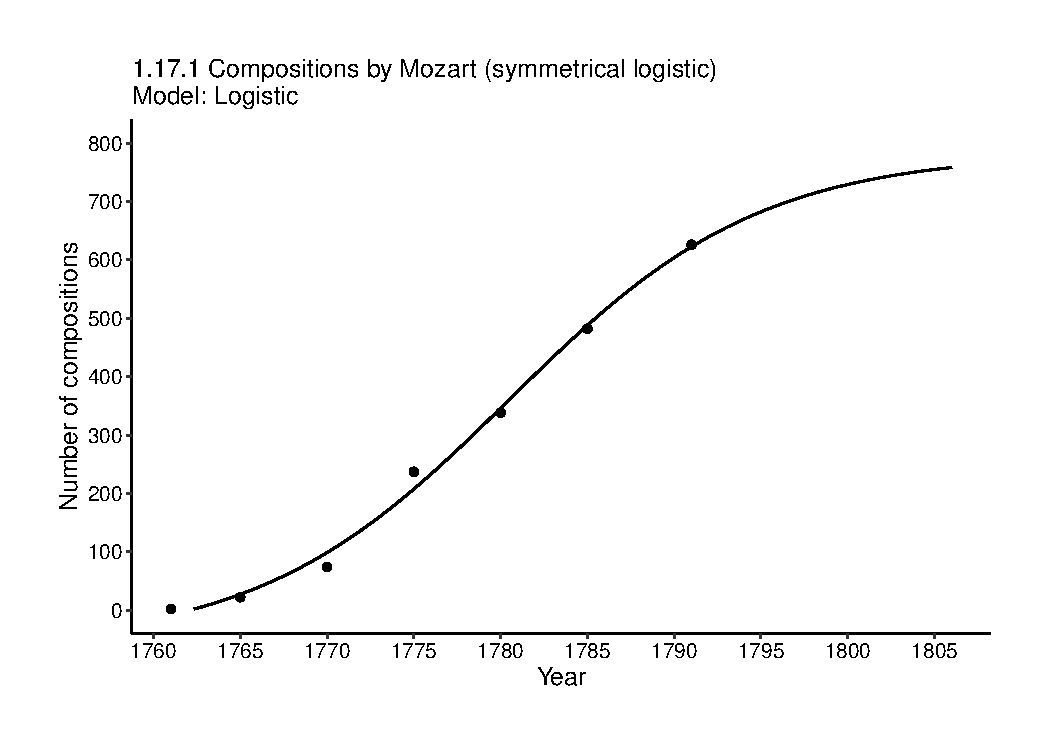
\includegraphics[width=8cm]{output/figs-ggplot/1.17.1.pdf}
\caption{\textbf{Dataset 1.17.1}: Fitting Mozart's oeuvre into growth curves: symmetrical (a)and asymmetrical (b) logistic functions and quadratic (c) and quartic (d) regression all have high degrees of fit (R^2=0.99) but predict substantially different long-term outcomes for the year 1806 when Mozart (who died in 1791) would have been 50 years old. Compositions by date listed in Giegling et al. (1964).}
\end{figure}
	
\begin{figure}[h]
\includegraphics[width=8cm]{output/figs-ggplot/1.17.2.pdf}
\caption{\textbf{Dataset 1.17.2}: Fitting Mozart's oeuvre into growth curves: symmetrical (a)and asymmetrical (b) logistic functions and quadratic (c) and quartic (d) regression all have high degrees of fit (R^2=0.99) but predict substantially different long-term outcomes for the year 1806 when Mozart (who died in 1791) would have been 50 years old. Compositions by date listed in Giegling et al. (1964).}
\end{figure}
	
\begin{figure}[h]
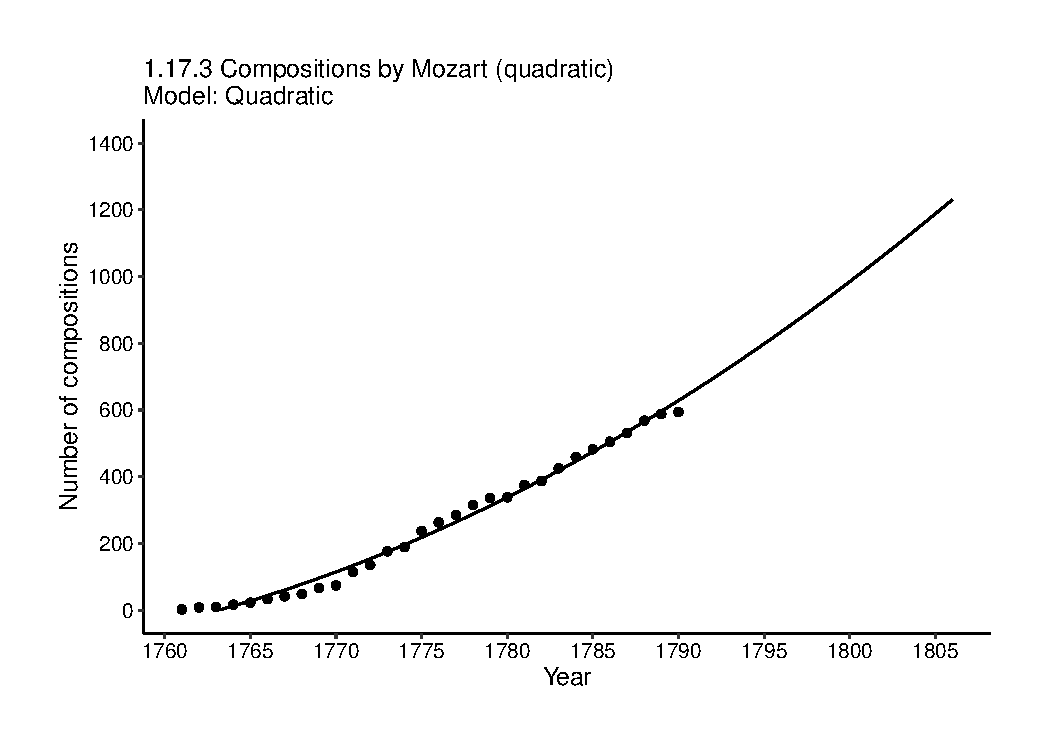
\includegraphics[width=8cm]{output/figs-ggplot/1.17.3.pdf}
\caption{\textbf{Dataset 1.17.3}: Fitting Mozart's oeuvre into growth curves: symmetrical (a)and asymmetrical (b) logistic functions and quadratic (c) and quartic (d) regression all have high degrees of fit (R^2=0.99) but predict substantially different long-term outcomes for the year 1806 when Mozart (who died in 1791) would have been 50 years old. Compositions by date listed in Giegling et al. (1964).}
\end{figure}
	
\begin{figure}[h]
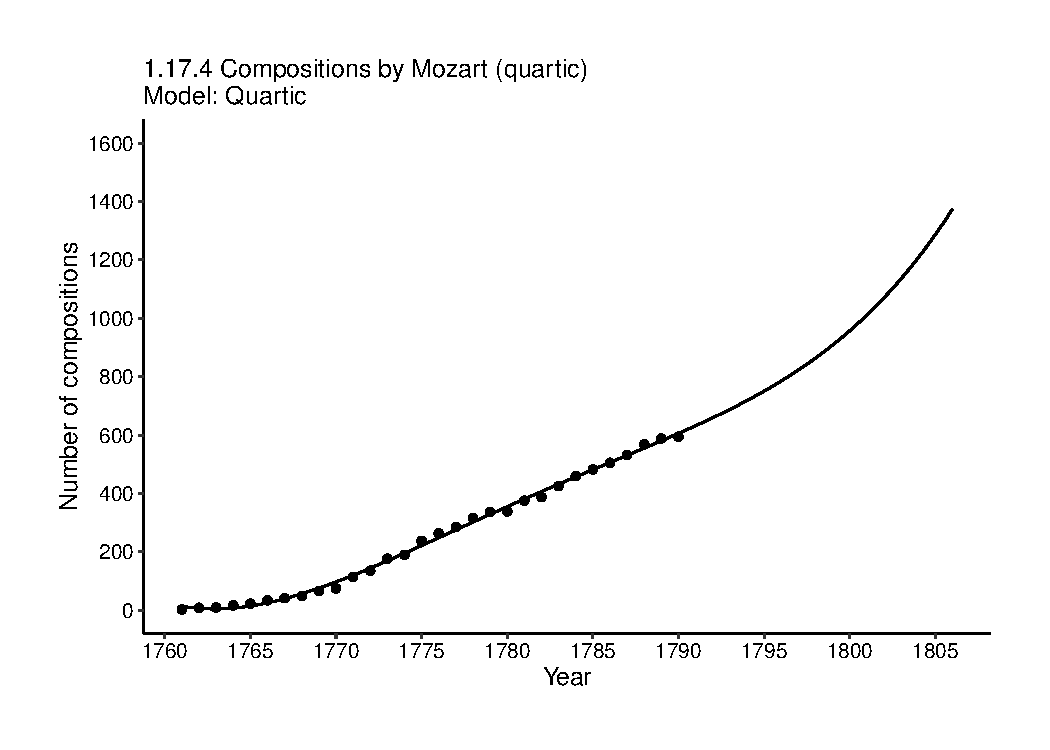
\includegraphics[width=8cm]{output/figs-ggplot/1.17.4.pdf}
\caption{\textbf{Dataset 1.17.4}: Fitting Mozart's oeuvre into growth curves: symmetrical (a)and asymmetrical (b) logistic functions and quadratic (c) and quartic (d) regression all have high degrees of fit (R^2=0.99) but predict substantially different long-term outcomes for the year 1806 when Mozart (who died in 1791) would have been 50 years old. Compositions by date listed in Giegling et al. (1964).}
\end{figure}
	
\begin{figure}[h]
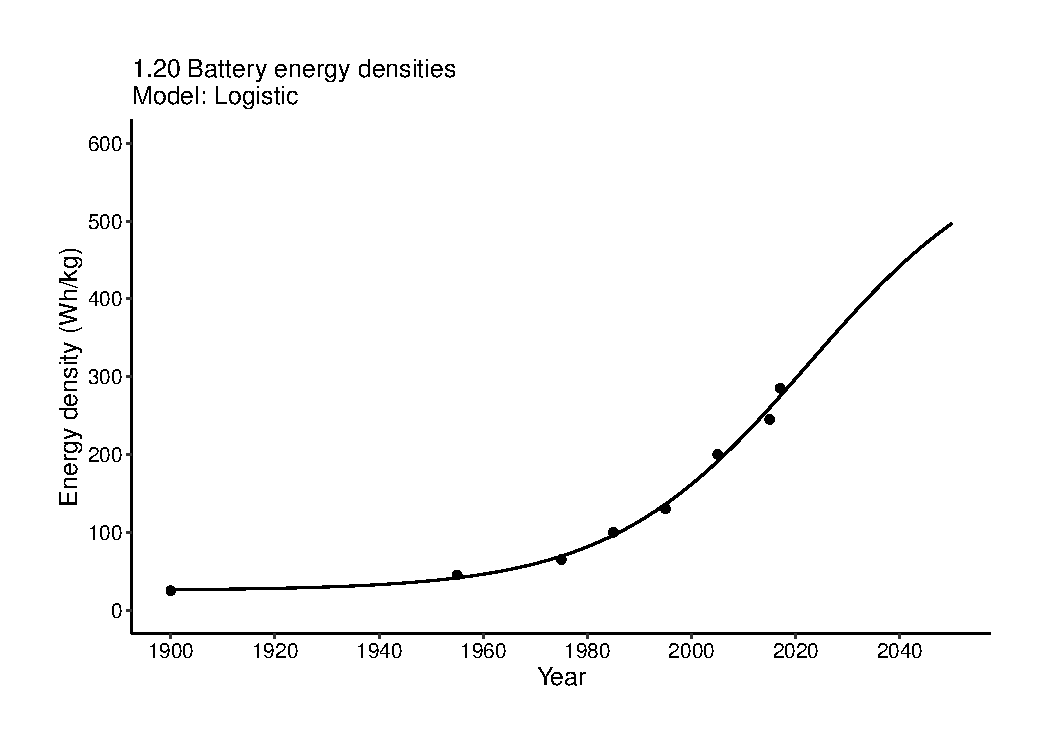
\includegraphics[width=8cm]{output/figs-ggplot/1.20.pdf}
\caption{\textbf{Dataset 1.20}: "Logistic growth trajectory (inflection point in 2024}
\end{figure}
	
\begin{figure}[h]
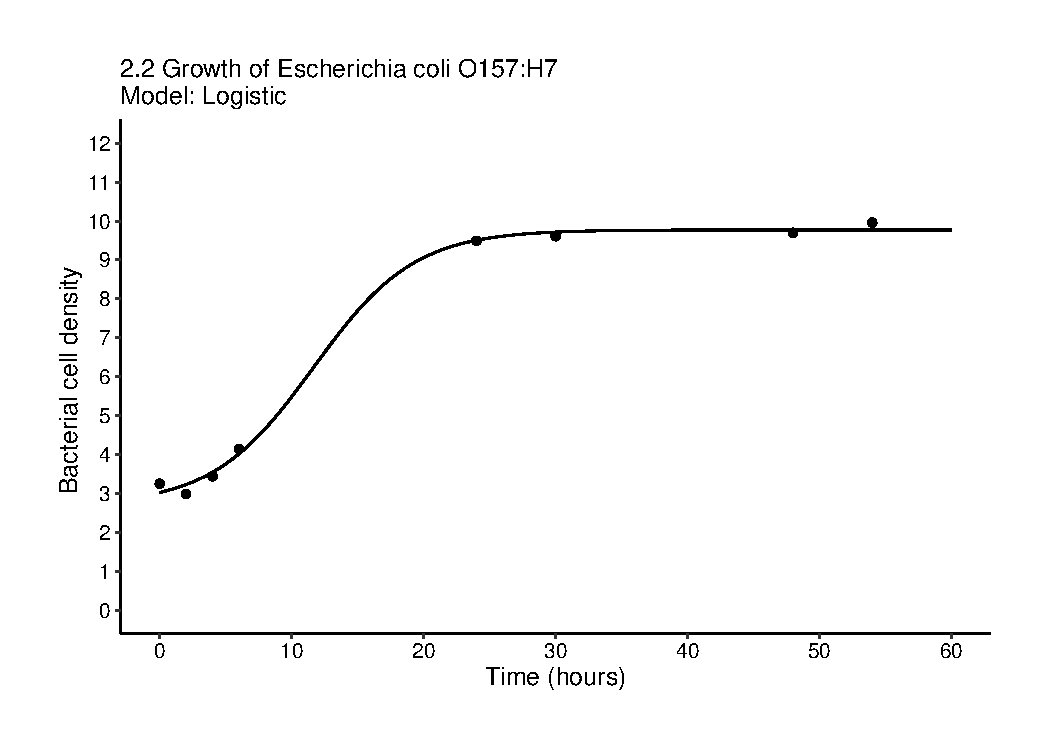
\includegraphics[width=8cm]{output/figs-ggplot/2.2.pdf}
\caption{\textbf{Dataset 2.2}: Logistic growth of Escherichia coli O157:H7. Plotted from data in Buchanan et al. (1997).}
\end{figure}
	
\begin{figure}[h]
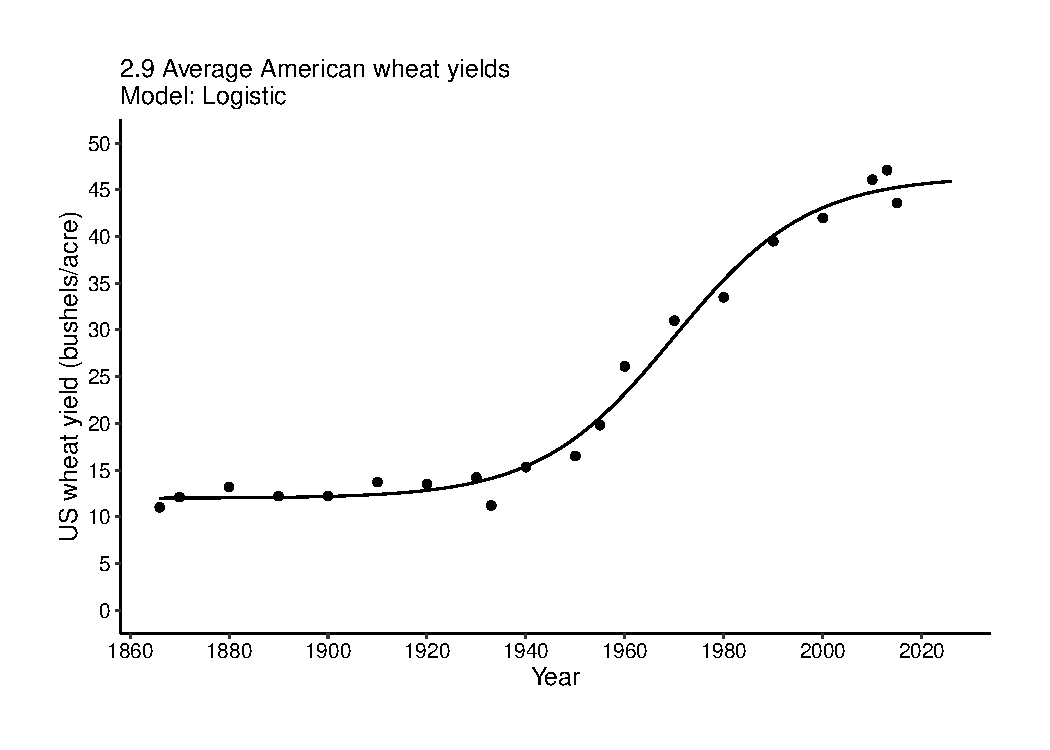
\includegraphics[width=8cm]{output/figs-ggplot/2.9.pdf}
\caption{\textbf{Dataset 2.9}: "Logistic growth (inflection point in 1970}
\end{figure}
	
\begin{figure}[h]
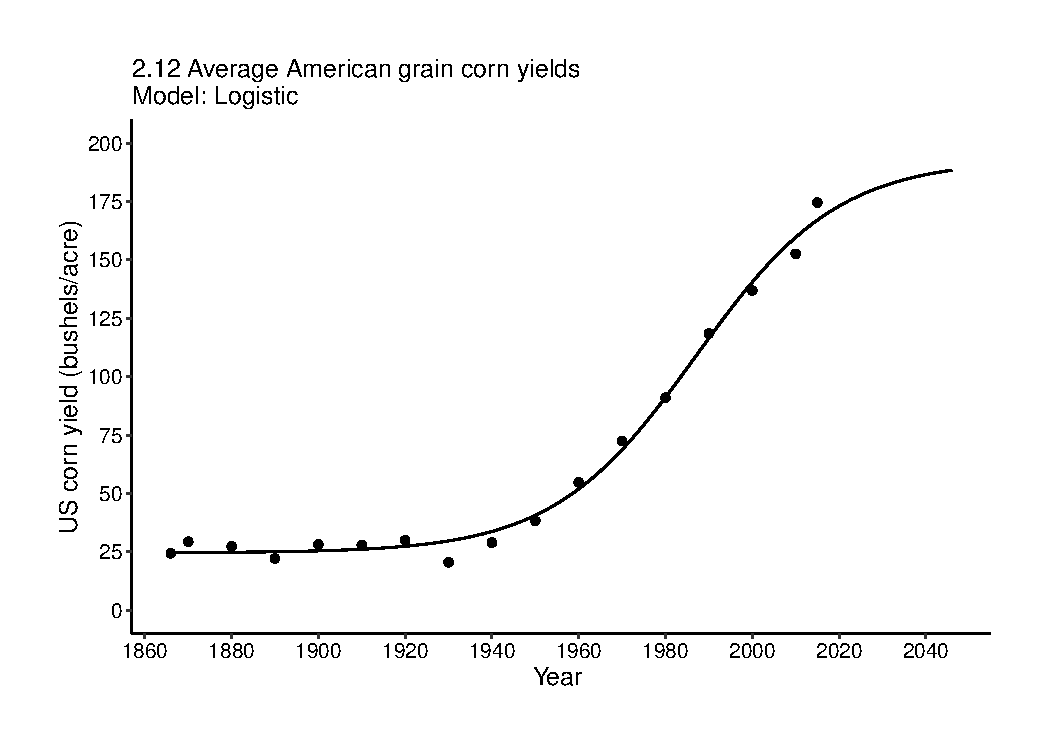
\includegraphics[width=8cm]{output/figs-ggplot/2.12.pdf}
\caption{\textbf{Dataset 2.12}: "Logistic growth trajectory (inflection point in 1988}
\end{figure}
	
\begin{figure}[h]
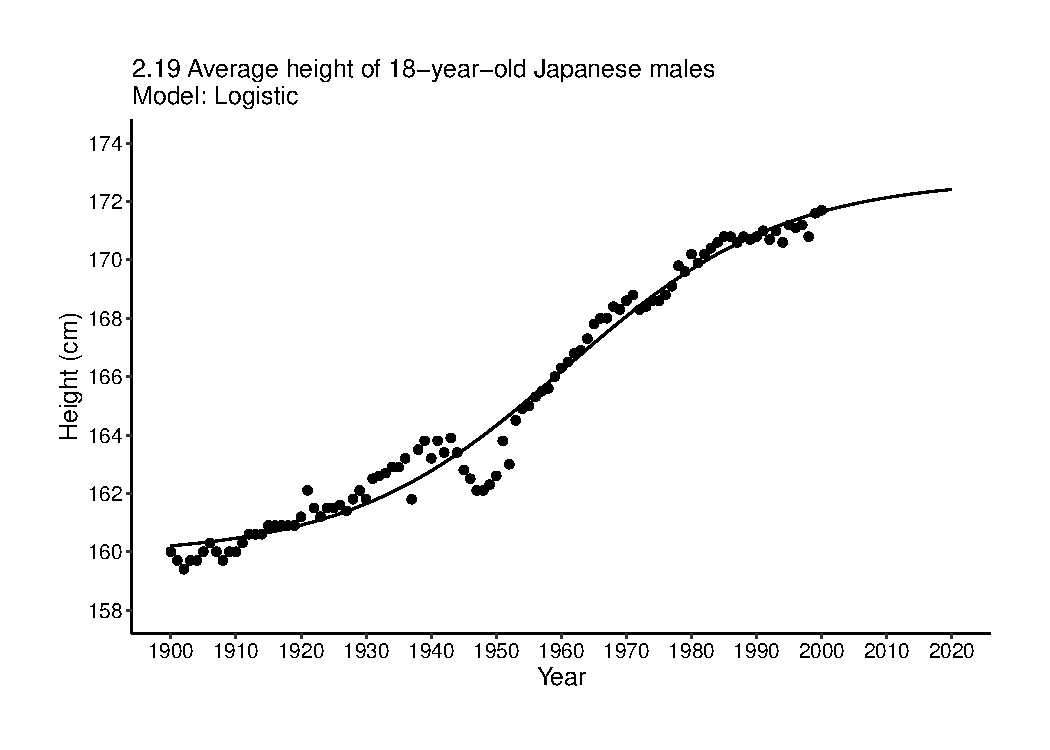
\includegraphics[width=8cm]{output/figs-ggplot/2.19.pdf}
\caption{\textbf{Dataset 2.19}: "Average height of 18-year-old Japanese males}
\end{figure}
	
\begin{figure}[h]
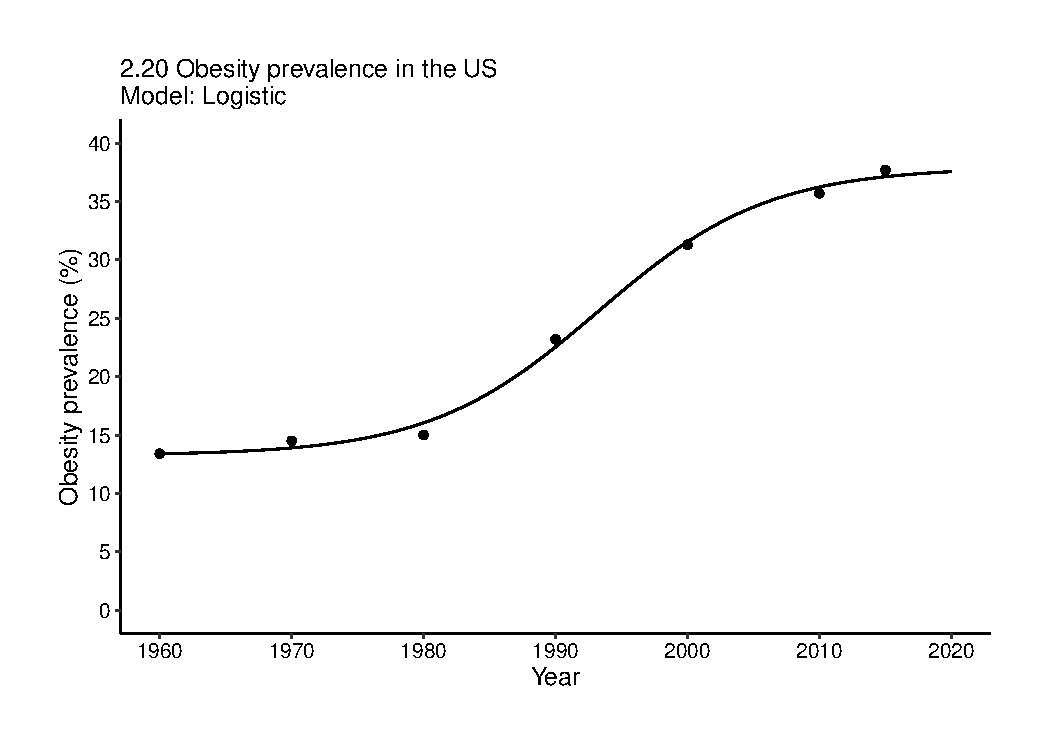
\includegraphics[width=8cm]{output/figs-ggplot/2.20.pdf}
\caption{\textbf{Dataset 2.20}: Growing prevalence of obesity in the US. Data from Ogden et al. (2012) and The State of Obesity (2012). The logistic curve had its inflection point in 1993 and its asymptote is at 37.5% of the total population.}
\end{figure}
	
\begin{figure}[h]
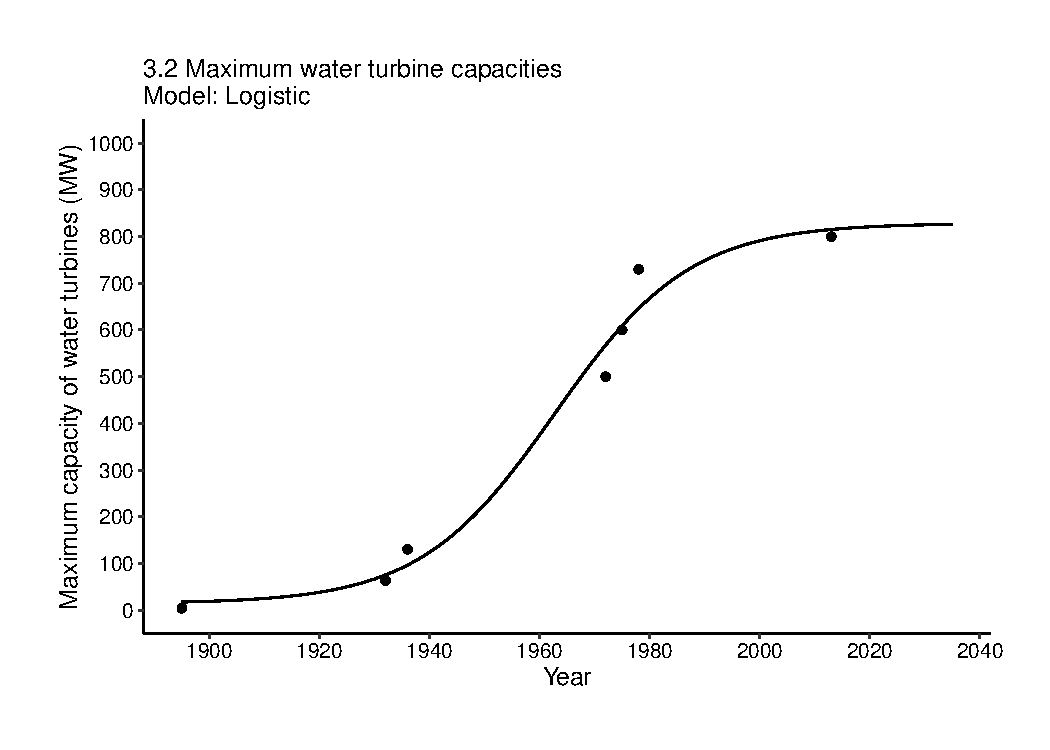
\includegraphics[width=8cm]{output/figs-ggplot/3.2.pdf}
\caption{\textbf{Dataset 3.2}: Logistic growth of maximum water turbine capacities since 1895; inflection point was in 1963. Data from Smil (2008) and ICOLD (2017).}
\end{figure}
	
\begin{figure}[h]
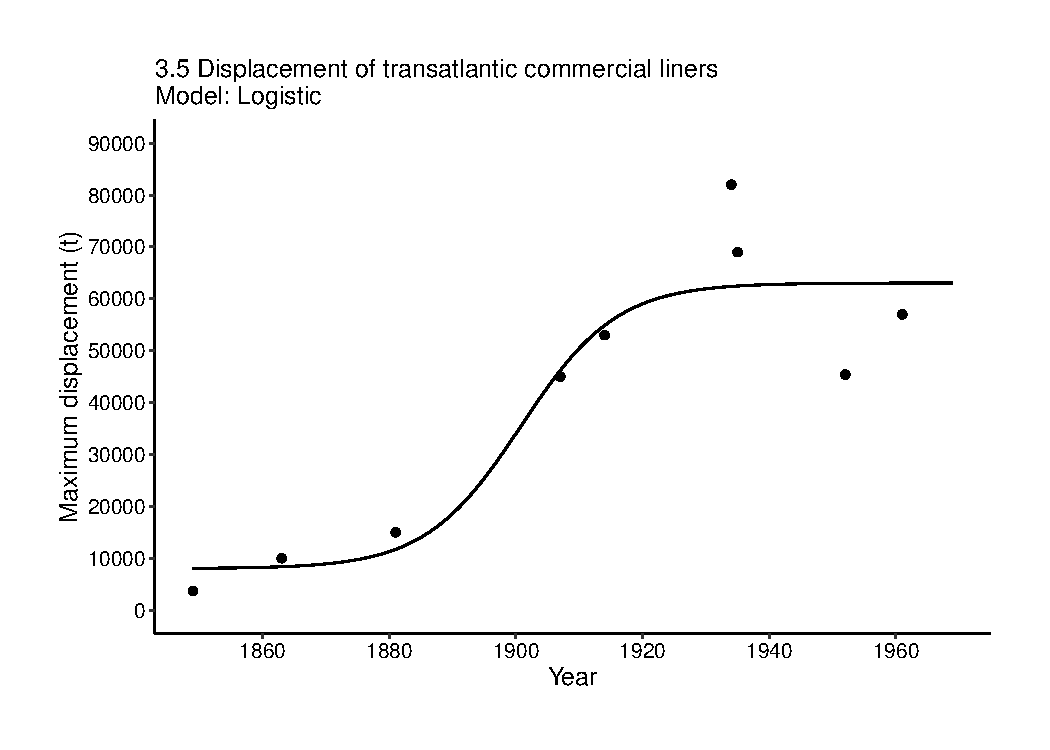
\includegraphics[width=8cm]{output/figs-ggplot/3.5.pdf}
\caption{\textbf{Dataset 3.5}: "Logistic curve of the maximum displacement of transatlantic commercial liners}
\end{figure}
	
\begin{figure}[h]
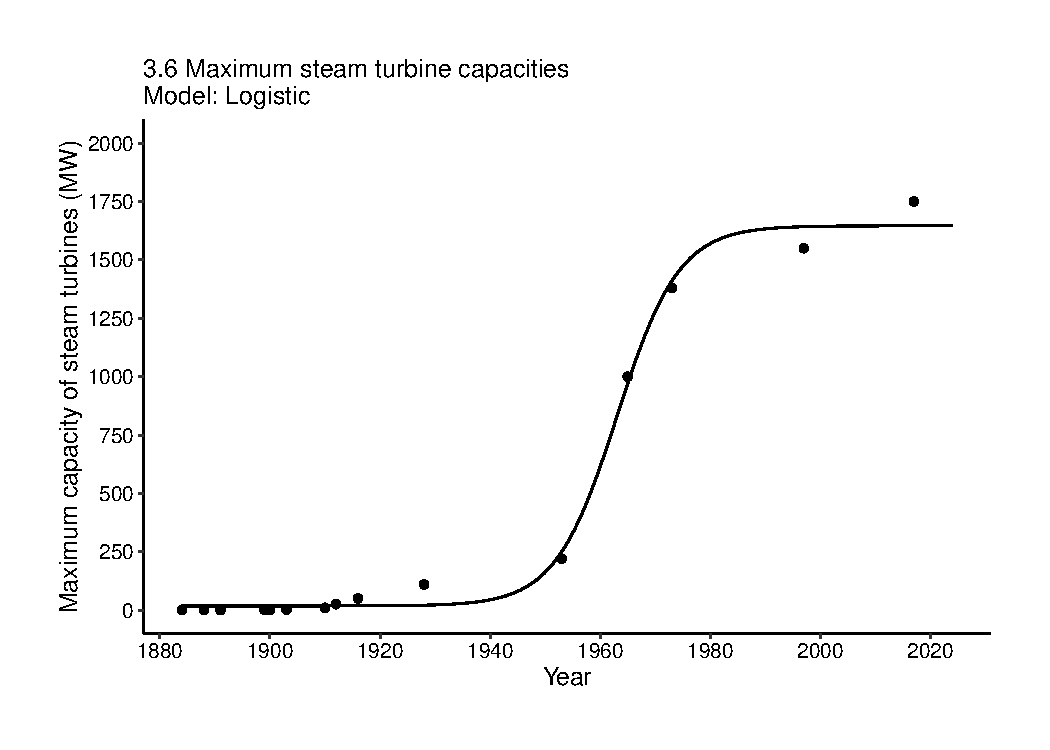
\includegraphics[width=8cm]{output/figs-ggplot/3.6.pdf}
\caption{\textbf{Dataset 3.6}: "Growth of maximum steam turbine capacities since 1884. Five-parameter [sic] logistic curve}
\end{figure}
	
\begin{figure}[h]
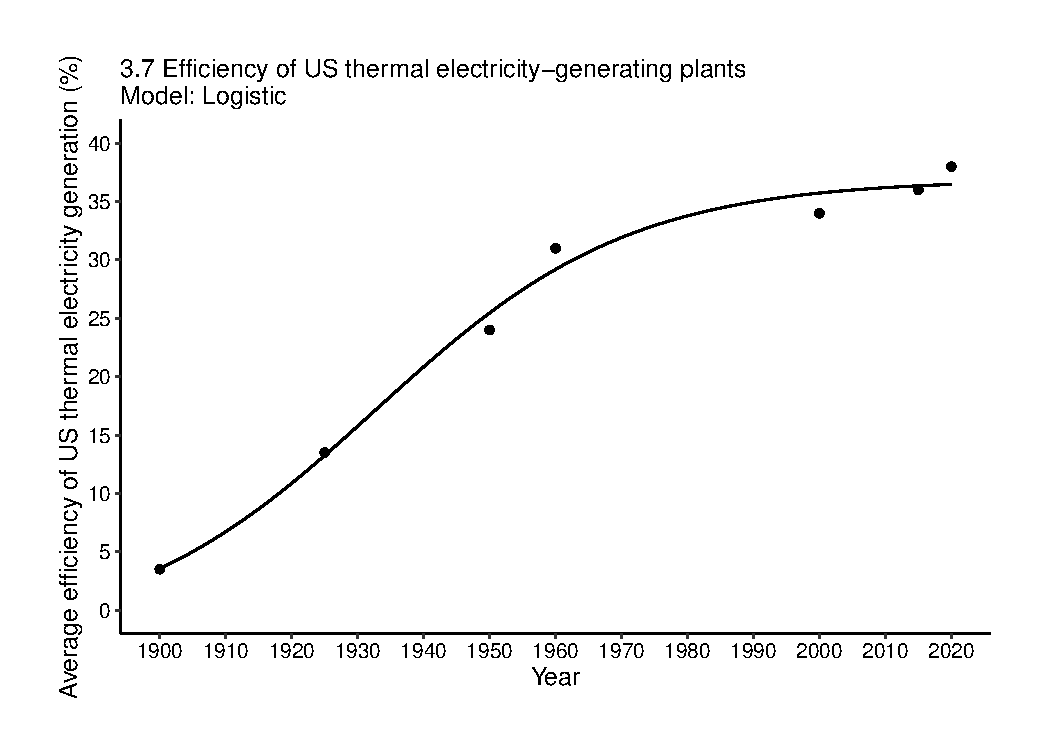
\includegraphics[width=8cm]{output/figs-ggplot/3.7.pdf}
\caption{\textbf{Dataset 3.7}: "Logistic growth (inflection year in 1933}
\end{figure}
	
\begin{figure}[h]
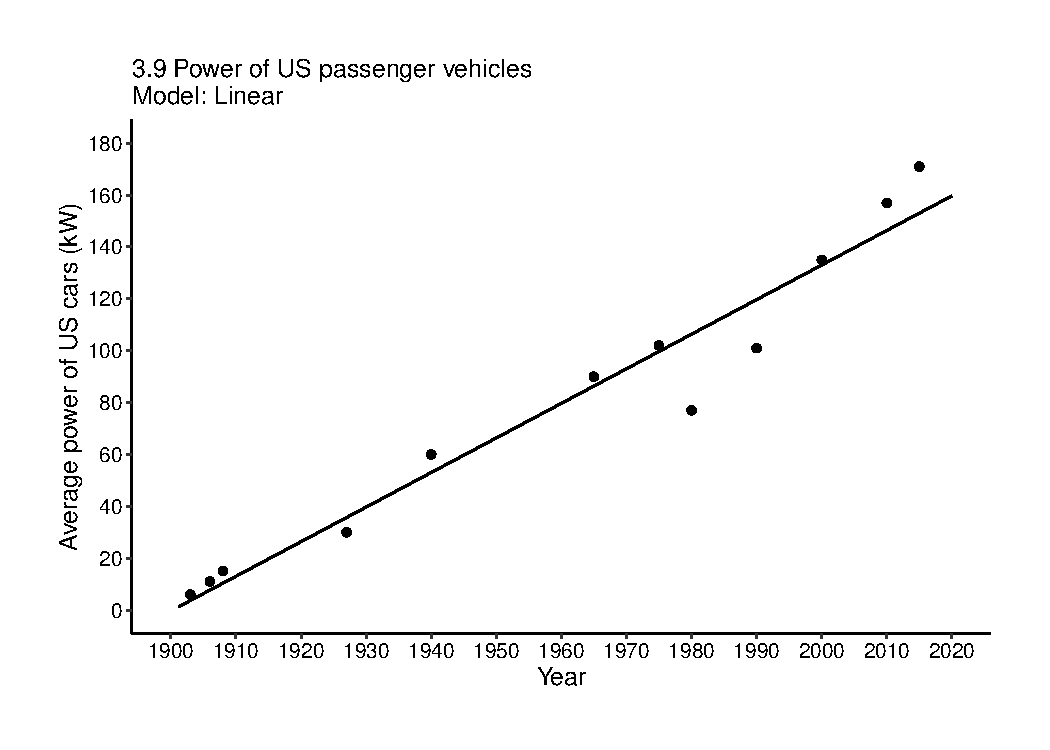
\includegraphics[width=8cm]{output/figs-ggplot/3.9.pdf}
\caption{\textbf{Dataset 3.9}: "Linear growth of average power of US passenger vehicles}
\end{figure}
	
\begin{figure}[h]
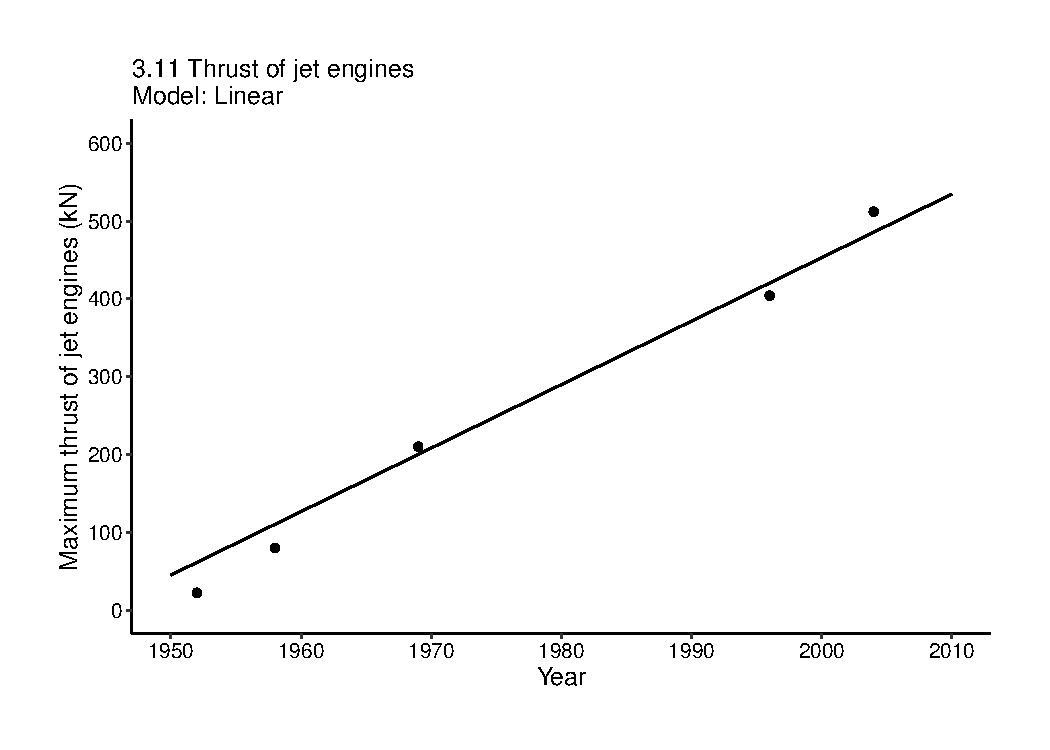
\includegraphics[width=8cm]{output/figs-ggplot/3.11.pdf}
\caption{\textbf{Dataset 3.11}: Linear fit of the maximum thrust of jet engines. Data from Smil (2010b).}
\end{figure}
	
\begin{figure}[h]
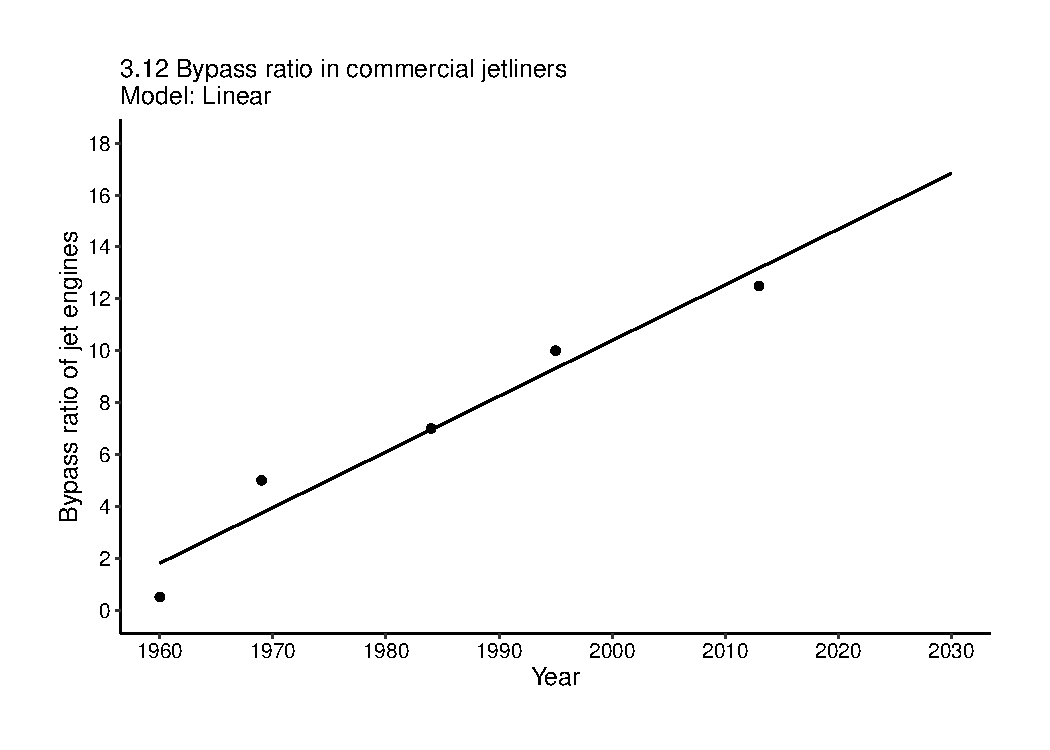
\includegraphics[width=8cm]{output/figs-ggplot/3.12.pdf}
\caption{\textbf{Dataset 3.12}: "Evolution of the bypass ratio in commercial jetliners. Data from specifications for GE}
\end{figure}
	
\begin{figure}[h]
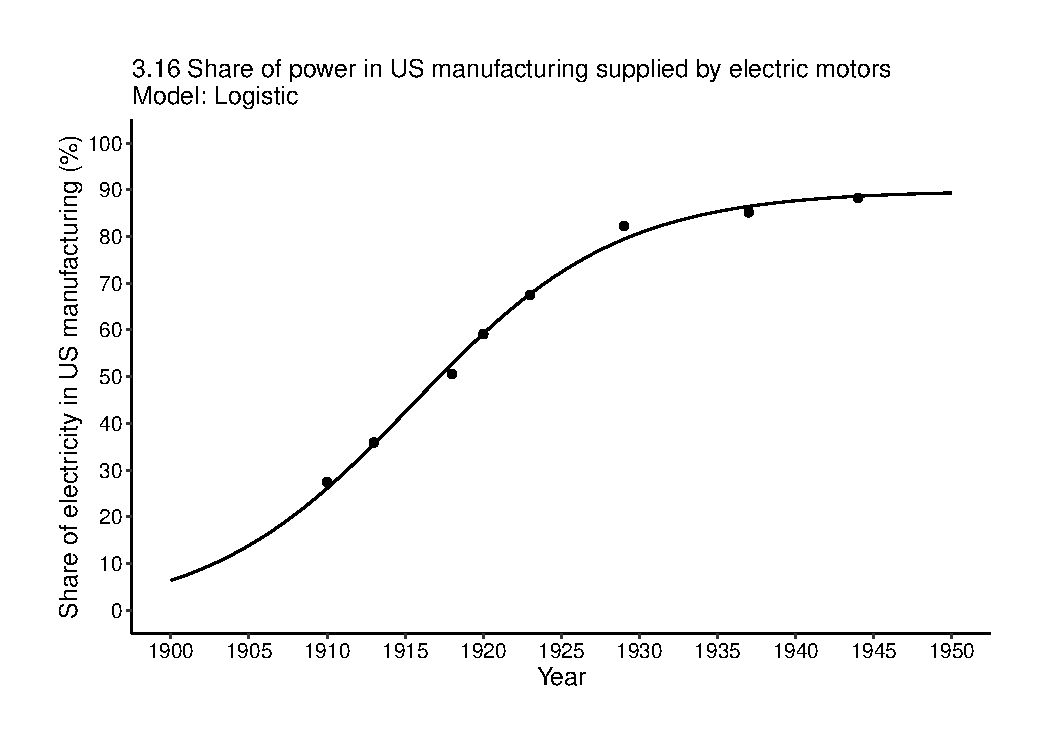
\includegraphics[width=8cm]{output/figs-ggplot/3.16.pdf}
\caption{\textbf{Dataset 3.16}: "Logistic fit (inflection point in 1916}
\end{figure}
	
\begin{figure}[h]
\includegraphics[width=8cm]{output/figs-ggplot/4.6.pdf}
\caption{\textbf{Dataset 4.6}: Logistic curve and polynomial regression of the growth of maximum skyscraper height. Data from Landau and Condit (1996) and Skyscraper Center (2017).}
\end{figure}
	
\begin{figure}[h]
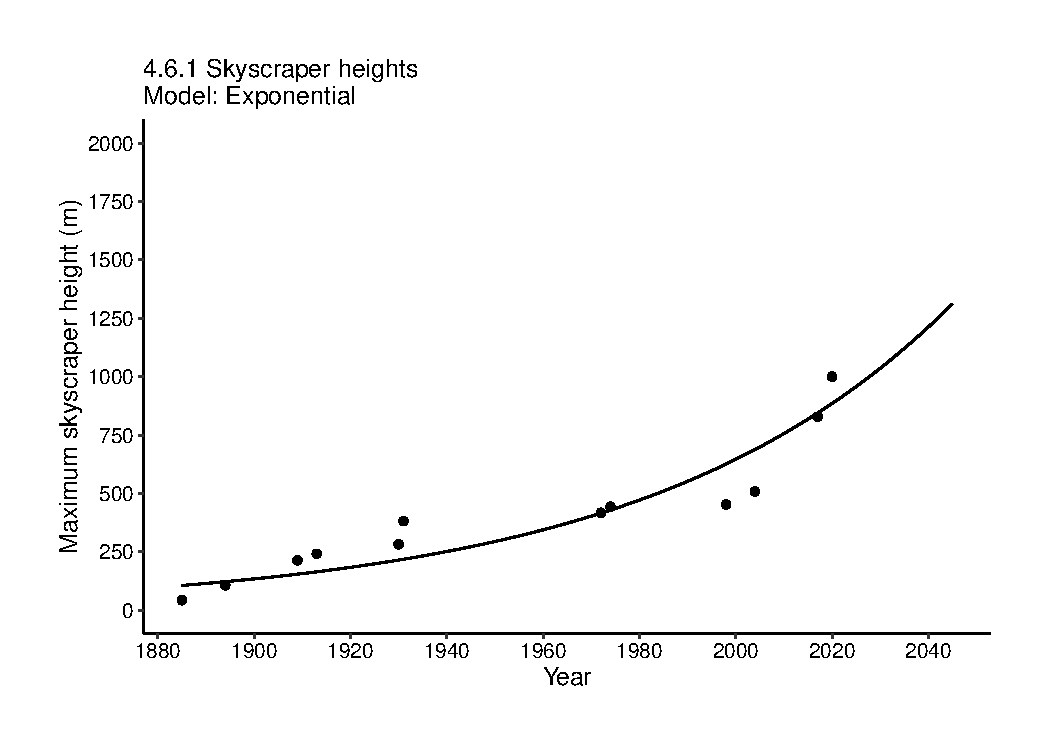
\includegraphics[width=8cm]{output/figs-ggplot/4.6.1.pdf}
\caption{\textbf{Dataset 4.6.1}: Logistic curve of the growth of maximum skyscraper height. Data from Landau and Condit (1996) and Skyscraper Center (2017).}
\end{figure}
	
\begin{figure}[h]
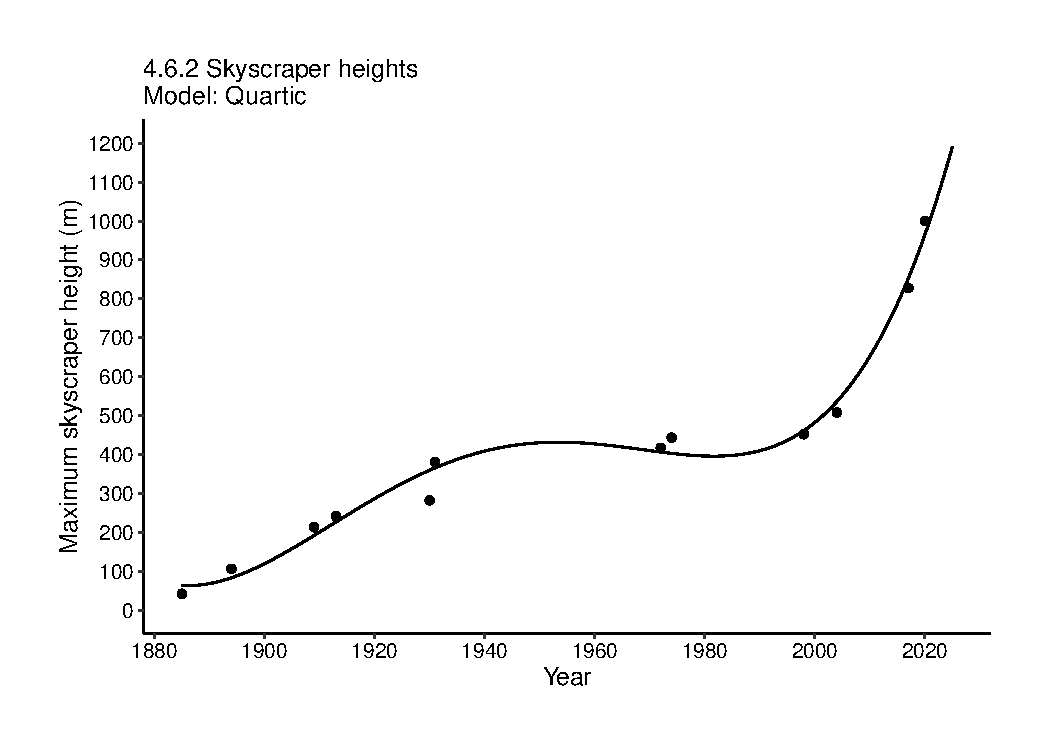
\includegraphics[width=8cm]{output/figs-ggplot/4.6.2.pdf}
\caption{\textbf{Dataset 4.6.2}: Polynomial regression of the growth of maximum skyscraper height. Data from Landau and Condit (1996) and Skyscraper Center (2017). }
\end{figure}
	
\begin{figure}[h]
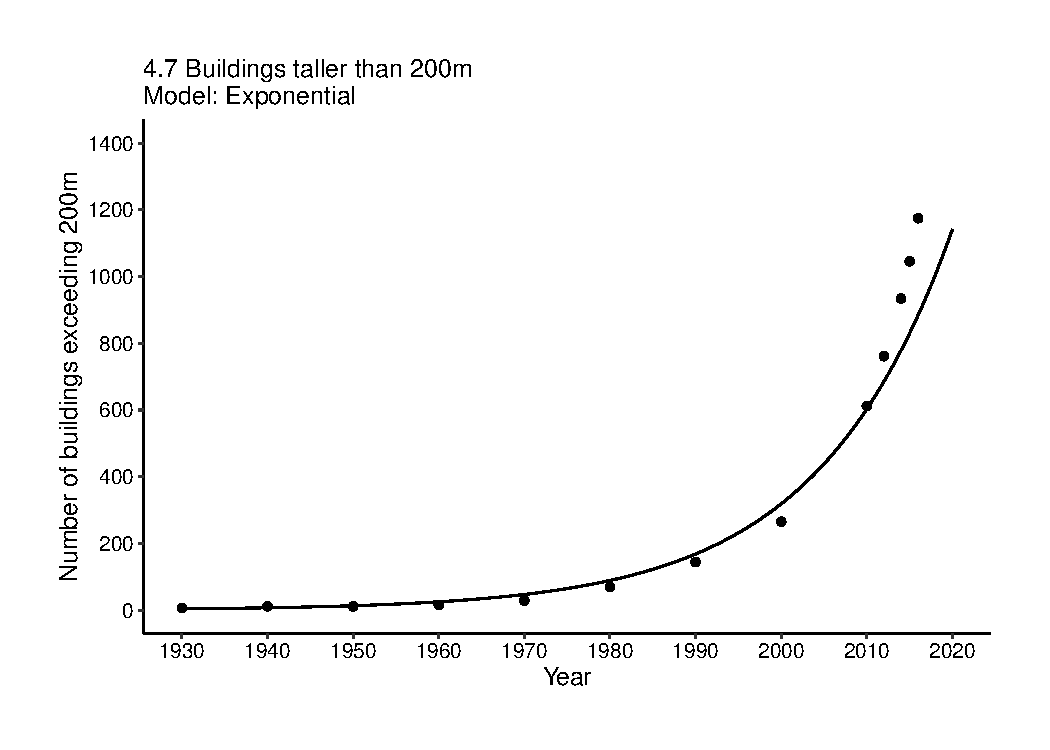
\includegraphics[width=8cm]{output/figs-ggplot/4.7.pdf}
\caption{\textbf{Dataset 4.7}: Growth of the total number of buildings taller than 200m. Logistic curve in its early stage of ascent. Data from Emporis (2017).}
\end{figure}
	
\begin{figure}[h]
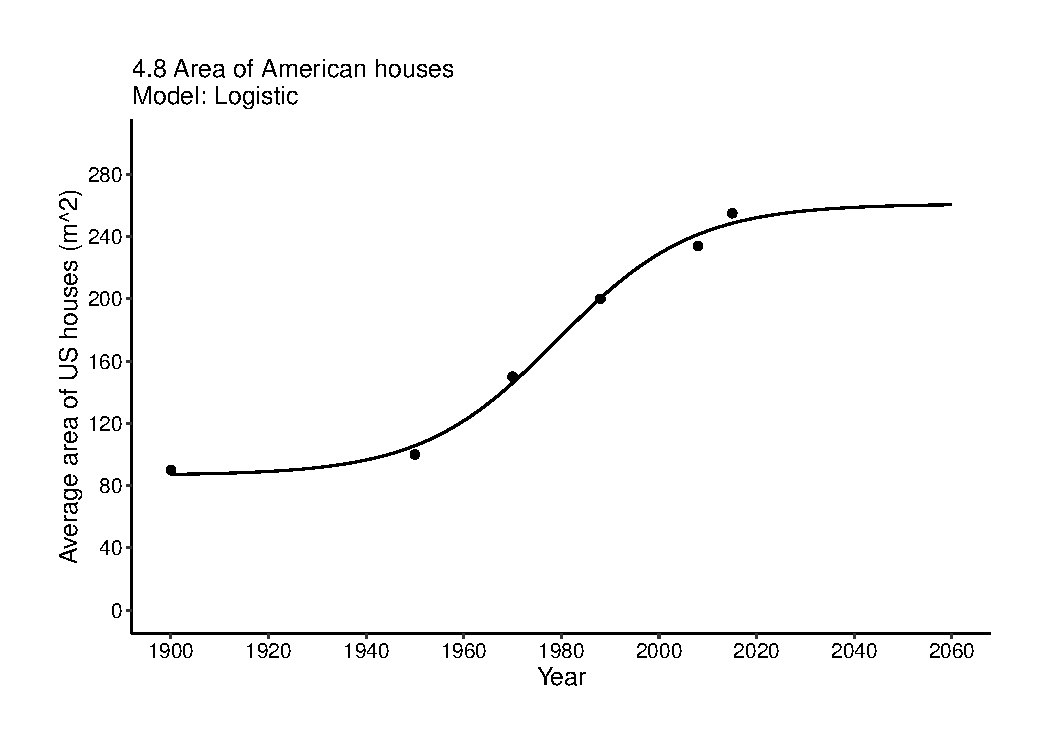
\includegraphics[width=8cm]{output/figs-ggplot/4.8.pdf}
\caption{\textbf{Dataset 4.8}: Growth of the average area of American houses since 1900. Logistic curve had the inflection year in 1979 and its asymptote is about 260 m^2. Data from Wilson and Boehland (2005) and USCB (2016a).}
\end{figure}
	
\begin{figure}[h]
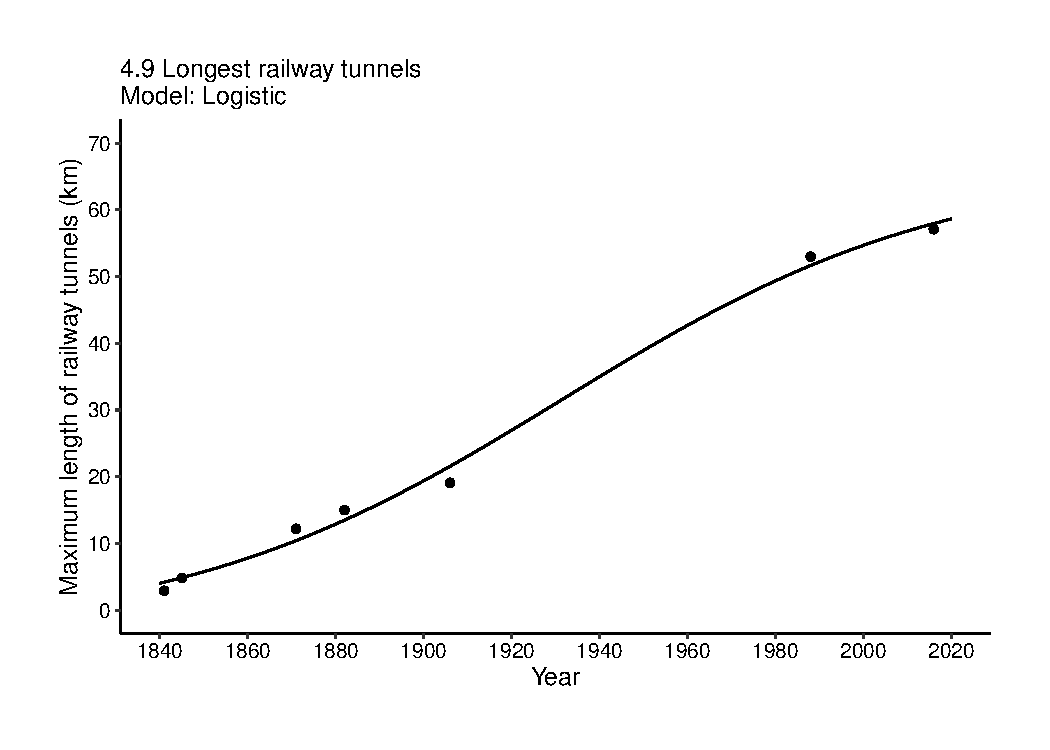
\includegraphics[width=8cm]{output/figs-ggplot/4.9.pdf}
\caption{\textbf{Dataset 4.9}: "Growth of the longest railway tunnels}
\end{figure}
	
\begin{figure}[h]
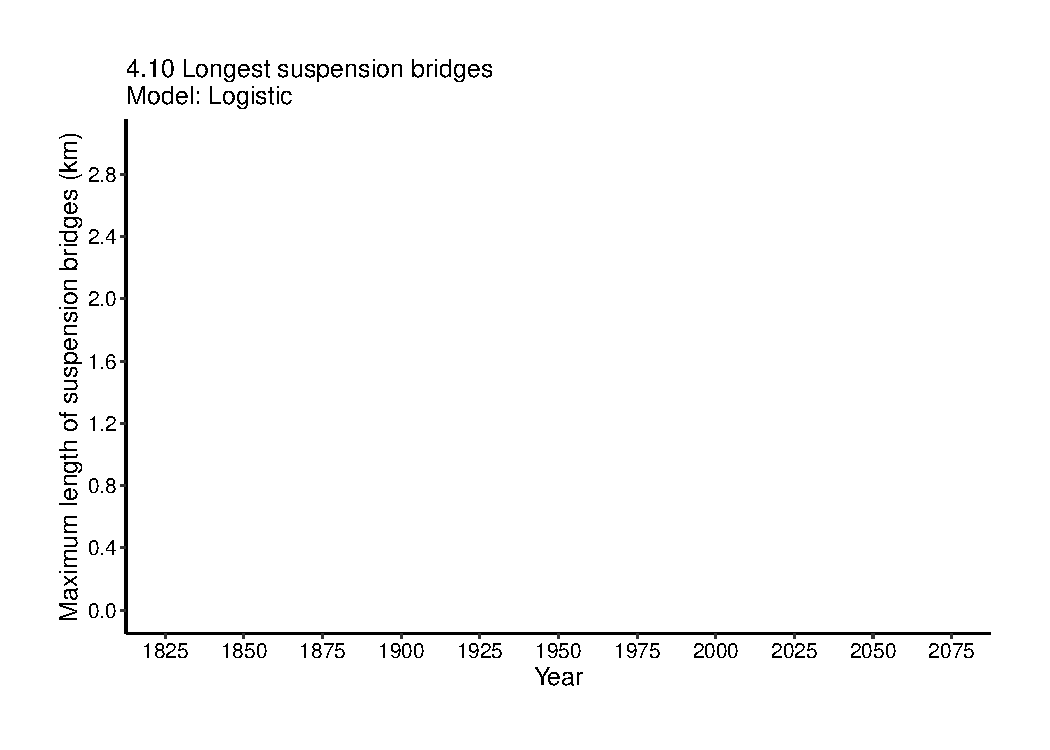
\includegraphics[width=8cm]{output/figs-ggplot/4.10.pdf}
\caption{\textbf{Dataset 4.10}: Growth of the longest suspension bridges since 1825. Data mostly from History of Bridges (2017).}
\end{figure}
	
\begin{figure}[h]
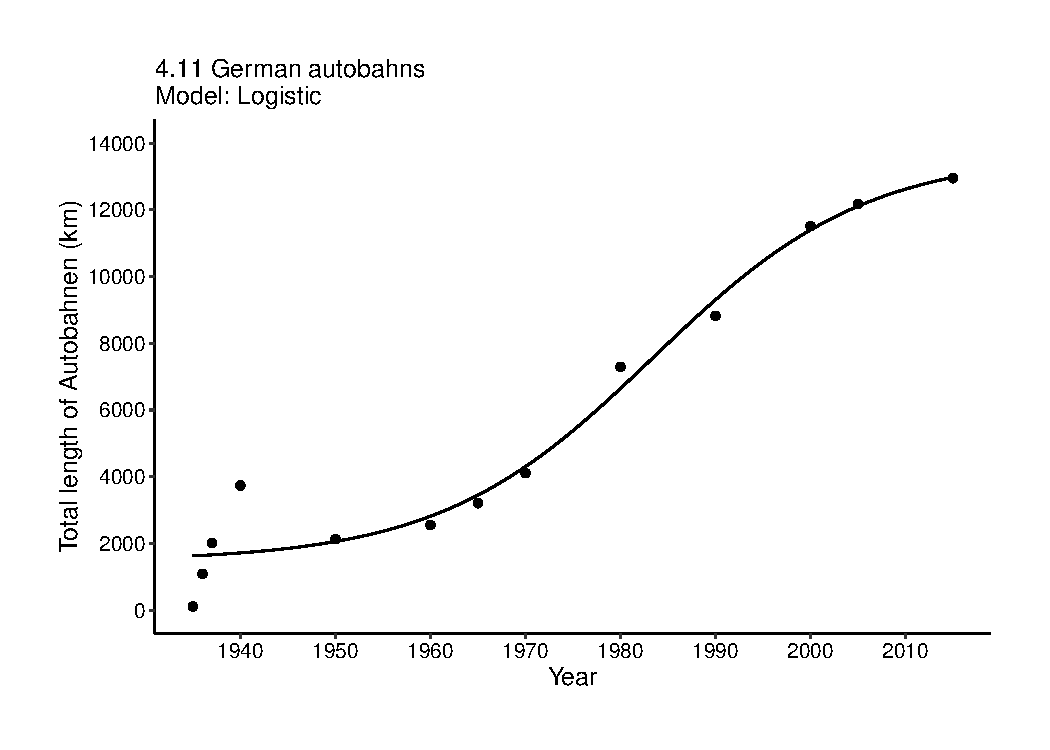
\includegraphics[width=8cm]{output/figs-ggplot/4.11.pdf}
\caption{\textbf{Dataset 4.11}: "Growth curve of German Autobahnen}
\end{figure}
	
\begin{figure}[h]
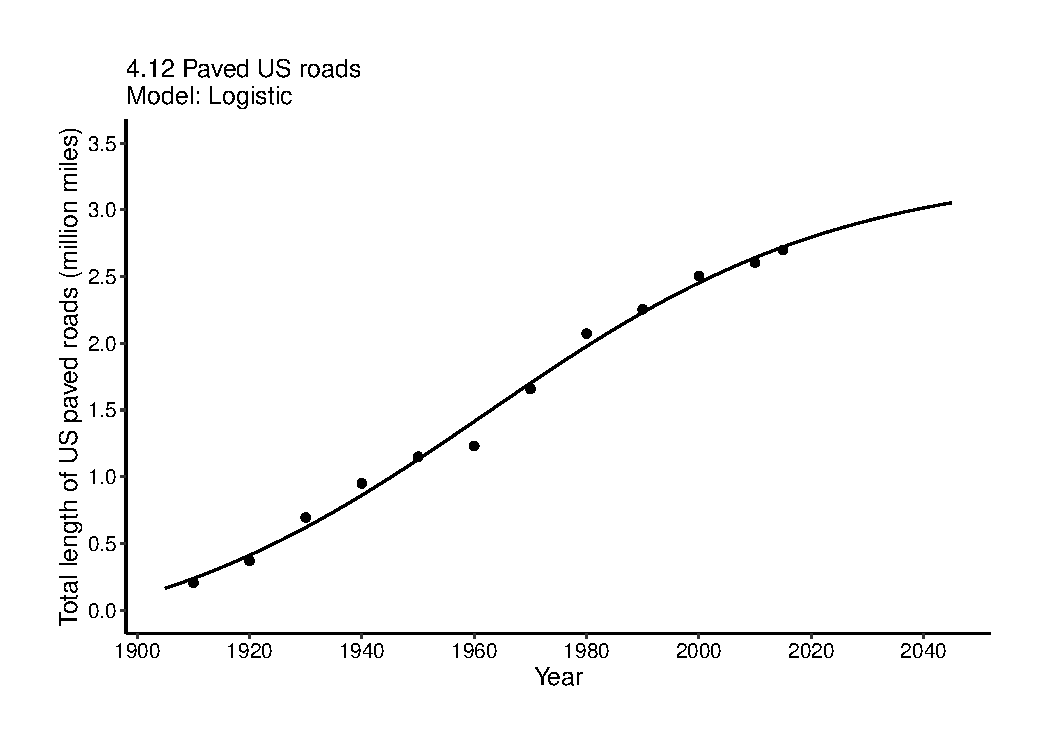
\includegraphics[width=8cm]{output/figs-ggplot/4.12.pdf}
\caption{\textbf{Dataset 4.12}: Growth of the total length of paved US roads since 1905. Plotted from data in USBC (1975) and subsequent volumes of US Statistical Abstract.}
\end{figure}
	
\begin{figure}[h]
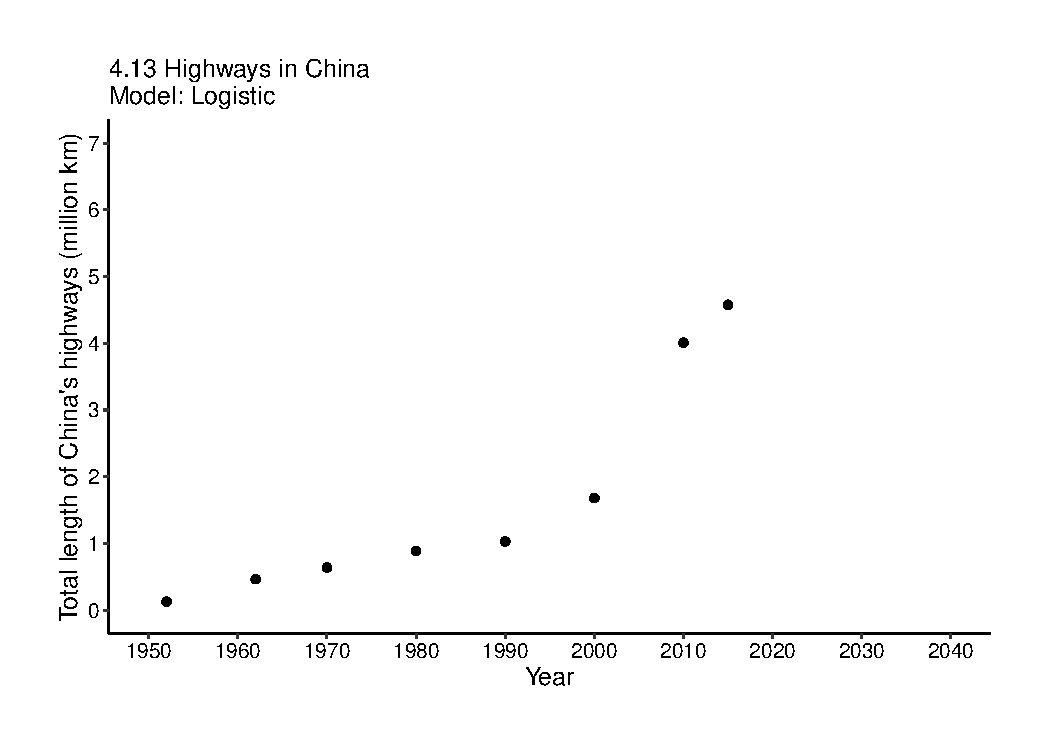
\includegraphics[width=8cm]{output/figs-ggplot/4.13.pdf}
\caption{\textbf{Dataset 4.13}: "Growth of the total length of highways in China. Logistic curve with the inflection point in 2007 and asymptote about 30% above the 2015 total. Data from NBS (2000}
\end{figure}
	
\begin{figure}[h]
\includegraphics[width=8cm]{output/figs-ggplot/4.14.pdf}
\caption{\textbf{Dataset 4.14}: "Growth curves of the total length of railroads in the US}
\end{figure}
	
\begin{figure}[h]
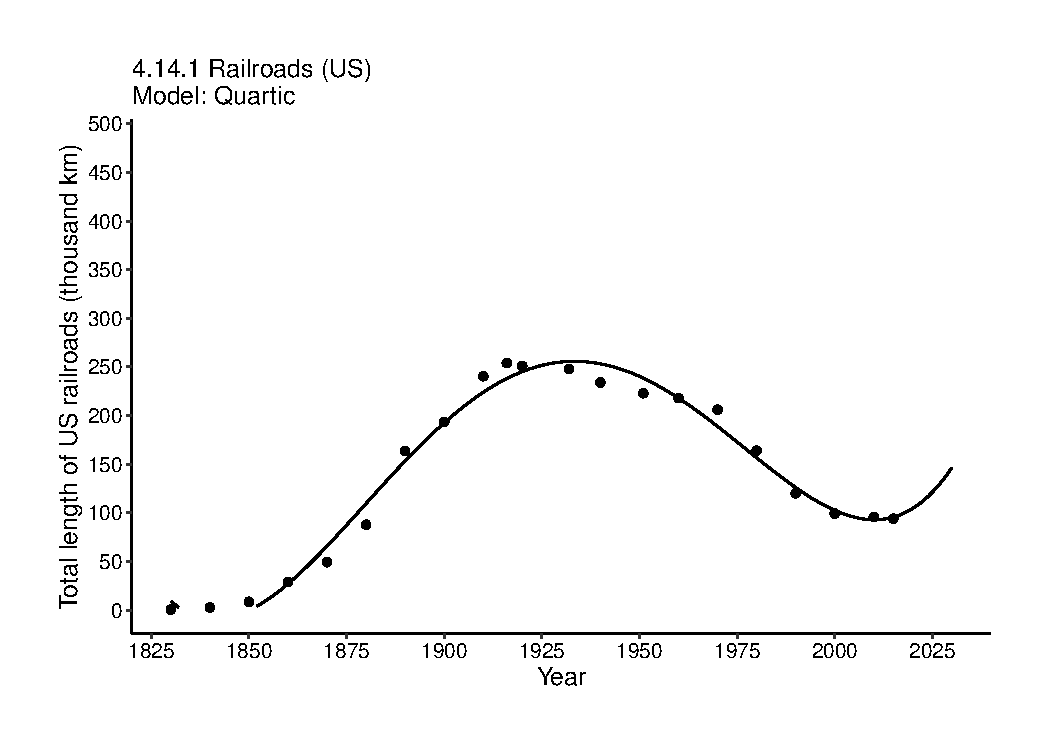
\includegraphics[width=8cm]{output/figs-ggplot/4.14.1.pdf}
\caption{\textbf{Dataset 4.14.1}: Growth curves of the total length of railroads in the US. Plotted from data in Mitchell (1998).}
\end{figure}
	
\begin{figure}[h]
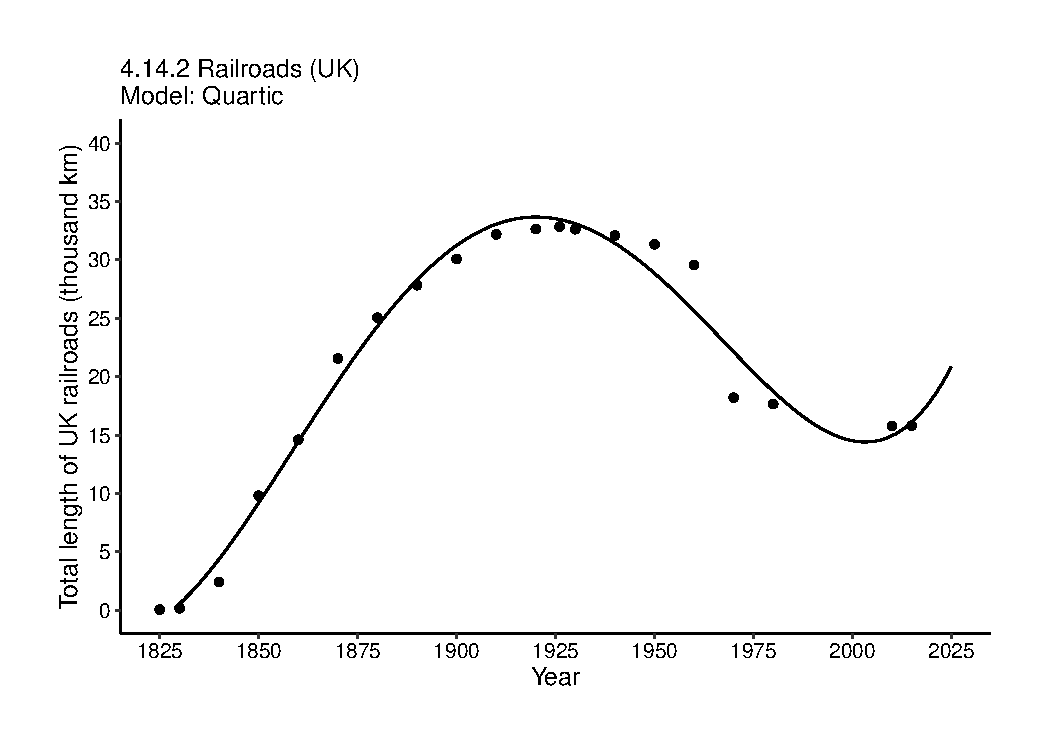
\includegraphics[width=8cm]{output/figs-ggplot/4.14.2.pdf}
\caption{\textbf{Dataset 4.14.2}: Growth curves of the total length of railroads in the UK. Plotted from data in Mitchell (1998).}
\end{figure}
	
\begin{figure}[h]
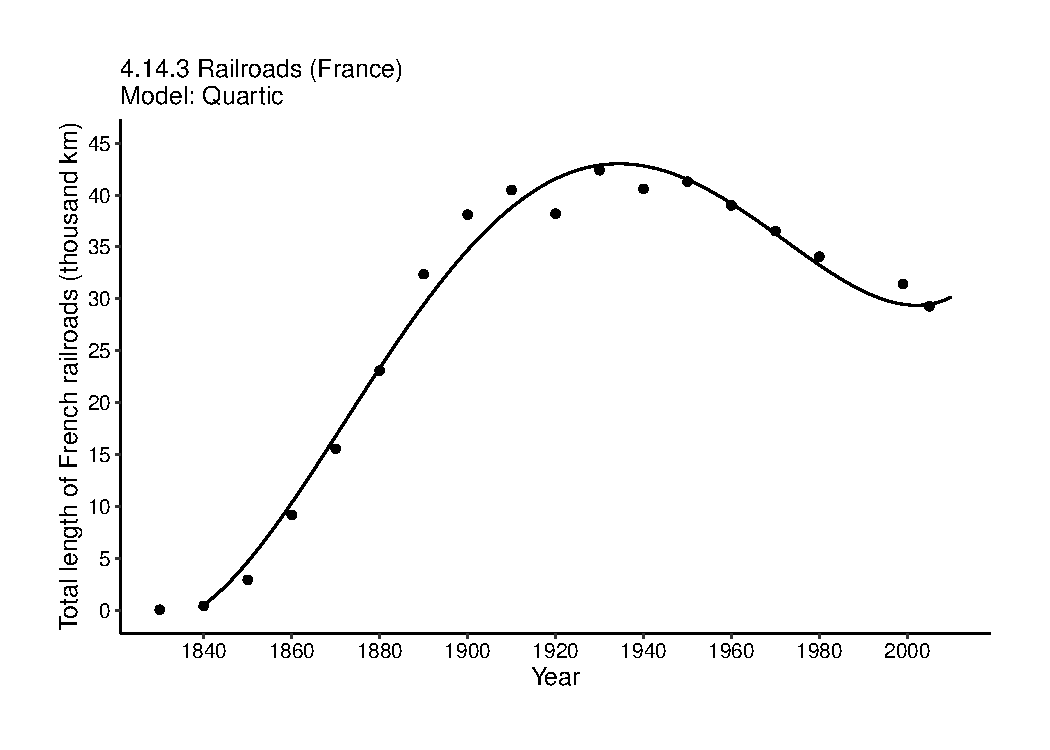
\includegraphics[width=8cm]{output/figs-ggplot/4.14.3.pdf}
\caption{\textbf{Dataset 4.14.3}: Growth curves of the total length of railroads in France. Plotted from data in Mitchell (1998).}
\end{figure}
	
\begin{figure}[h]
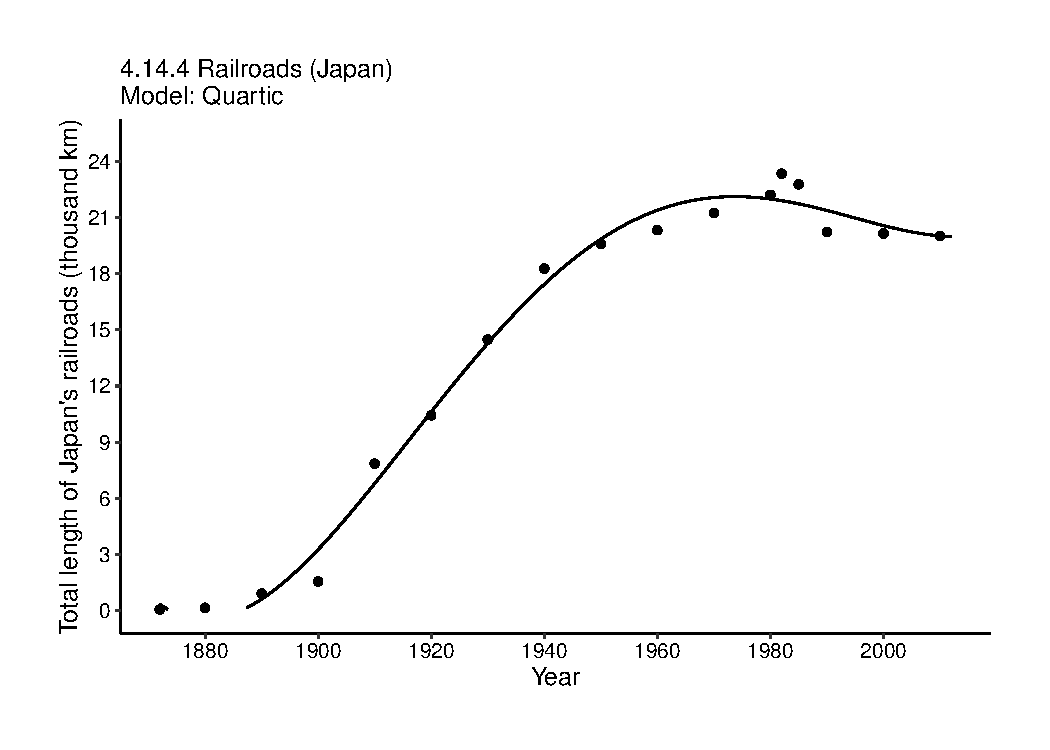
\includegraphics[width=8cm]{output/figs-ggplot/4.14.4.pdf}
\caption{\textbf{Dataset 4.14.4}: Growth curves of the total length of railroads in Japan. Plotted from data in Mitchell (1998).}
\end{figure}
	
\begin{figure}[h]
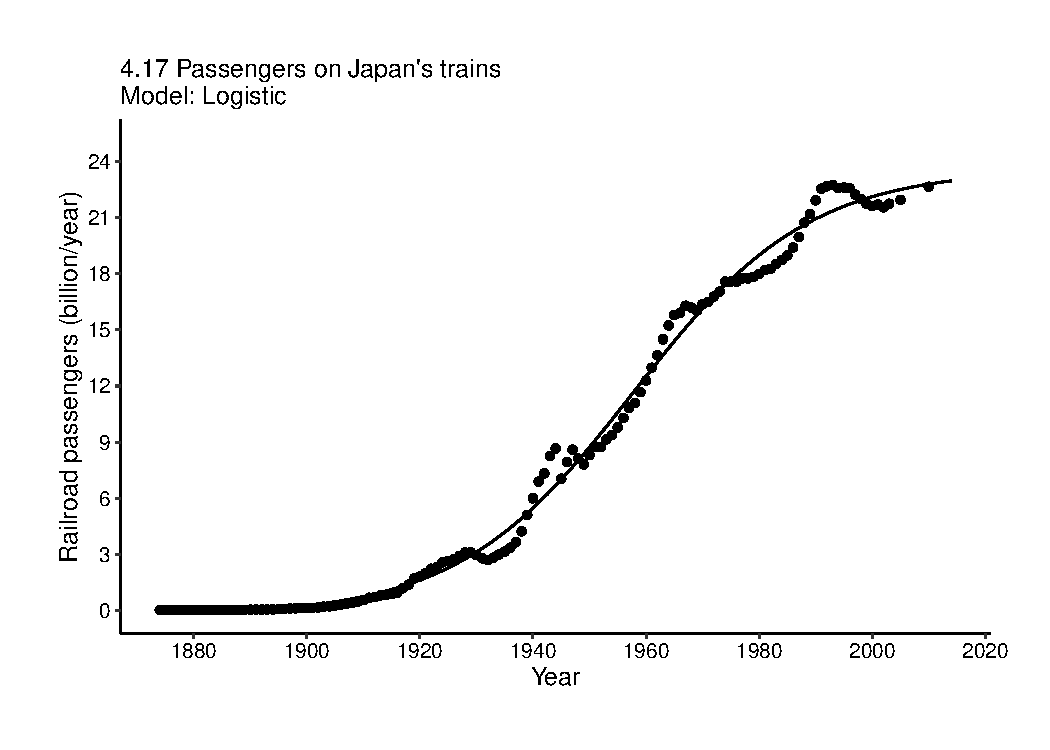
\includegraphics[width=8cm]{output/figs-ggplot/4.17.pdf}
\caption{\textbf{Dataset 4.17}: "Passengers on Japan's trains}
\end{figure}
	
\begin{figure}[h]
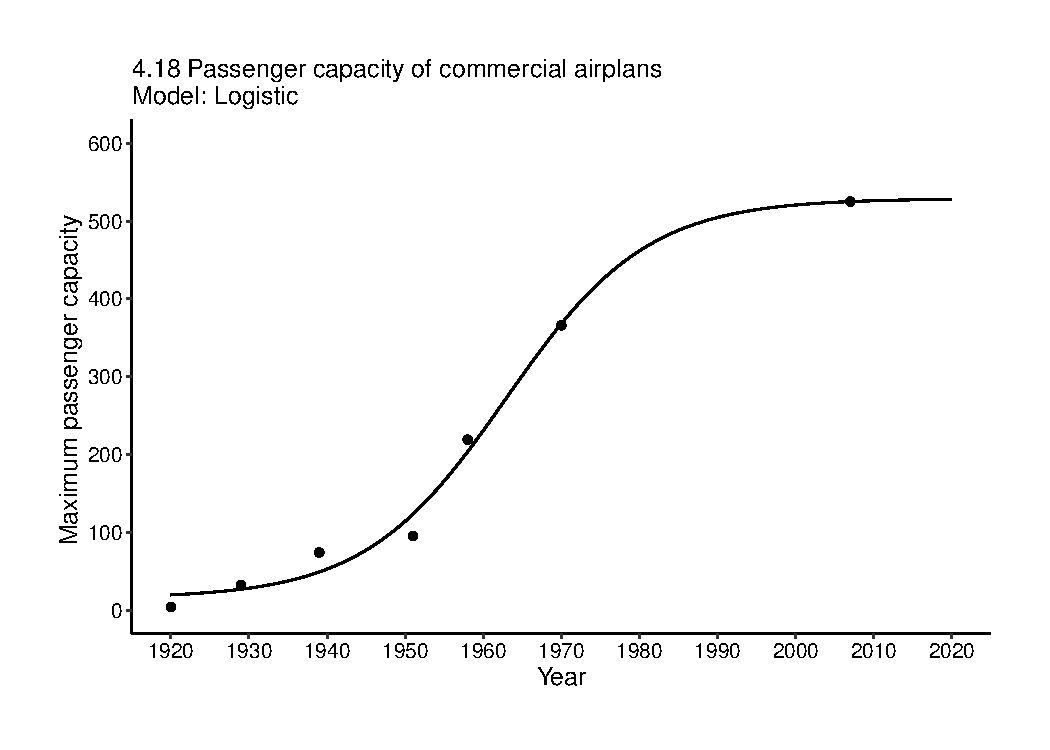
\includegraphics[width=8cm]{output/figs-ggplot/4.18.pdf}
\caption{\textbf{Dataset 4.18}: "Logistic fit of the maximum passenger capacity of commercial airplans: from KLM's de Havilland DH.16 (four passengers) in 1920 to Airbus 380 (544 passengers in three classes}
\end{figure}
	
\begin{figure}[h]
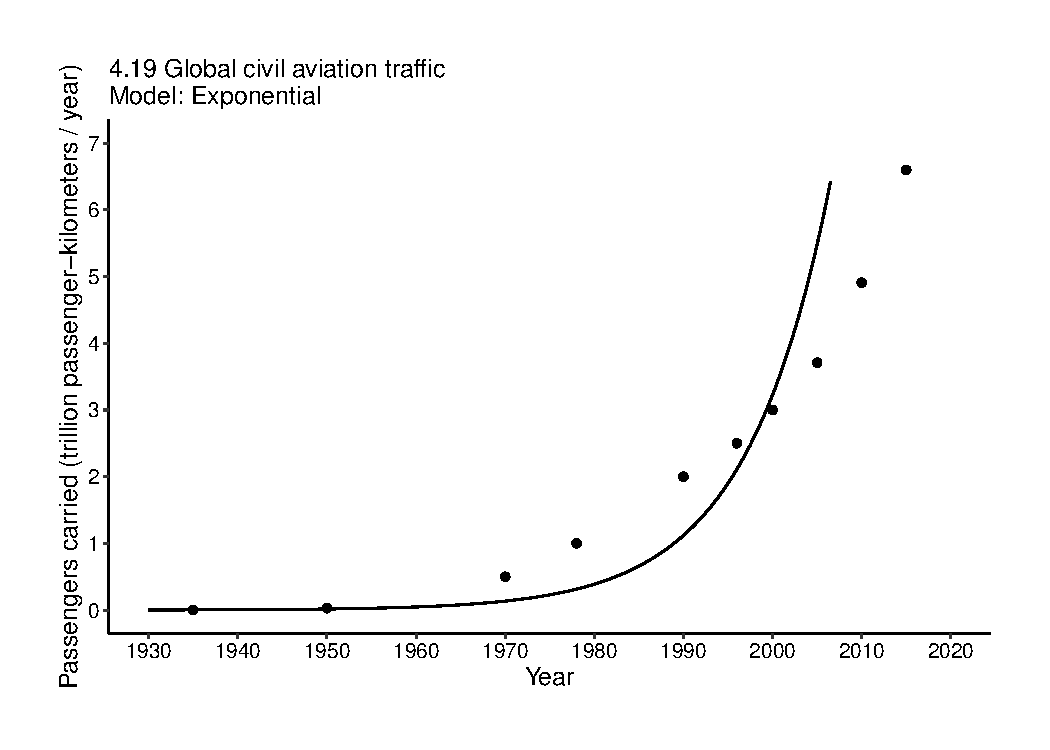
\includegraphics[width=8cm]{output/figs-ggplot/4.19.pdf}
\caption{\textbf{Dataset 4.19}: Growth of global civil aviation traffic (domestic and international flights) measured in terms of passenger-kilometers. Logistic curve in its early stage indicates further substantial growth in the decades ahead. Data from ICAO (2016) and from earlier annual reports. }
\end{figure}
	
\begin{figure}[h]
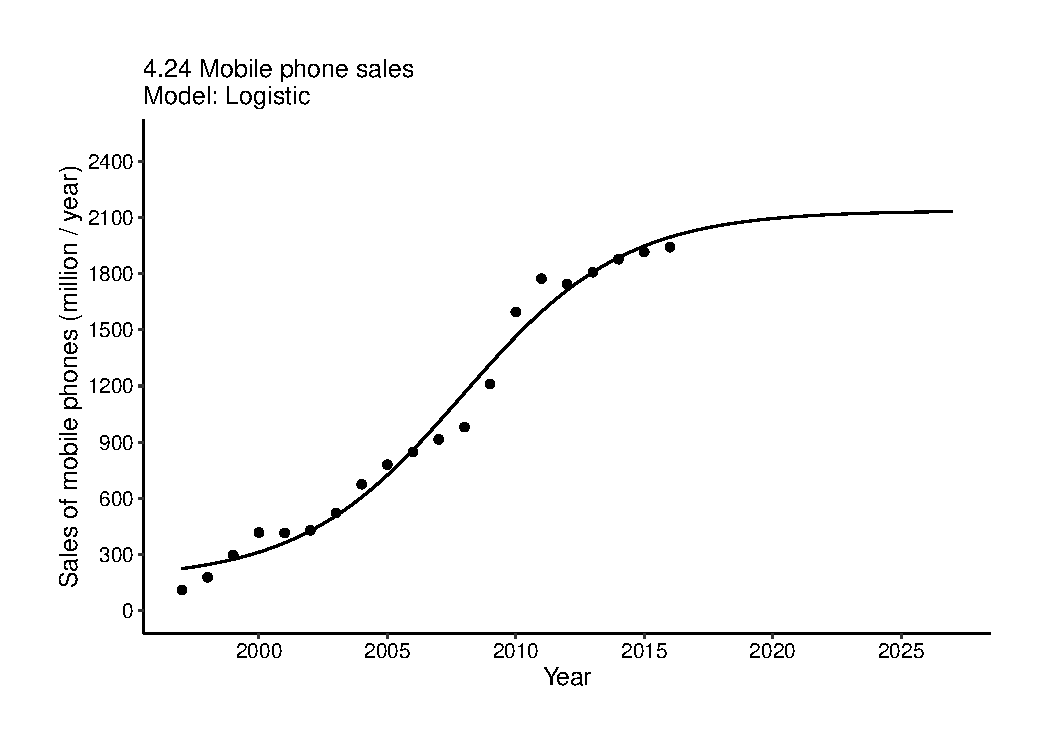
\includegraphics[width=8cm]{output/figs-ggplot/4.24.pdf}
\caption{\textbf{Dataset 4.24}: Growth of annual sales of all mobile phones since 1997. The trajectory fits a logistic curve that inflected in 2008 and that is now approaching its asymptotic value. Data from GSMArena (2017).}
\end{figure}
	
\begin{figure}[h]
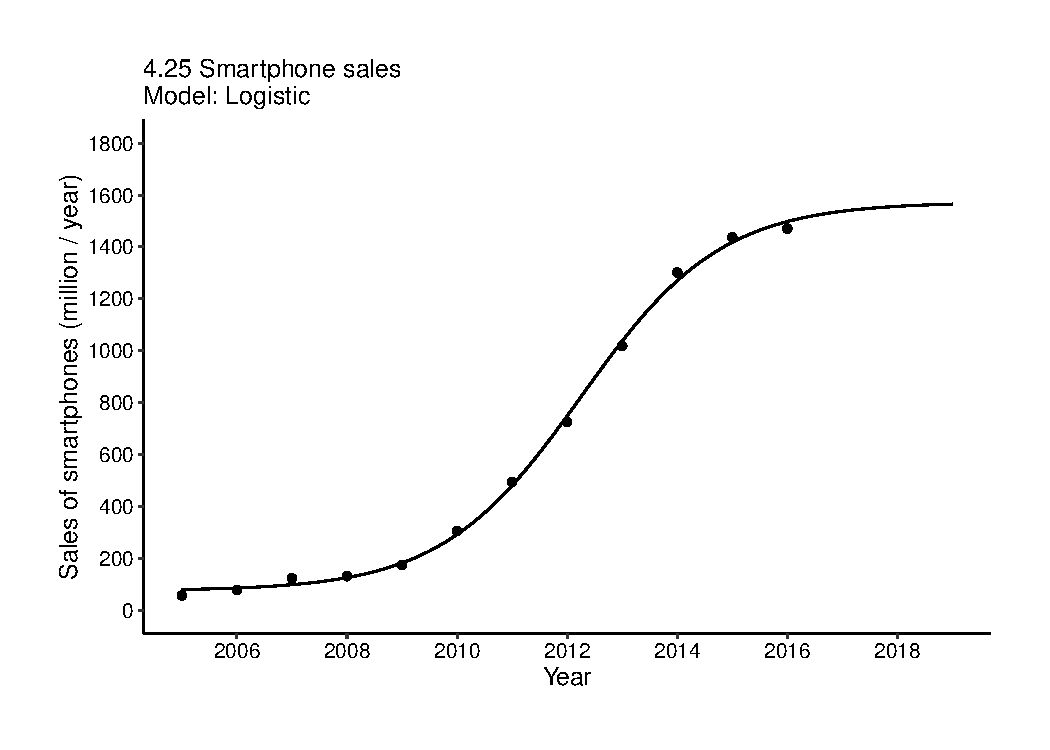
\includegraphics[width=8cm]{output/figs-ggplot/4.25.pdf}
\caption{\textbf{Dataset 4.25}: The growth of annual sales of smartphones since the year 2005 has followed perfectly a logistic curve with the inflection year in 2012 and with the asymptote less than 10% above 2016 sales. Data from Canalys (2007) and Meeker (2017).}
\end{figure}
	
\begin{figure}[h]
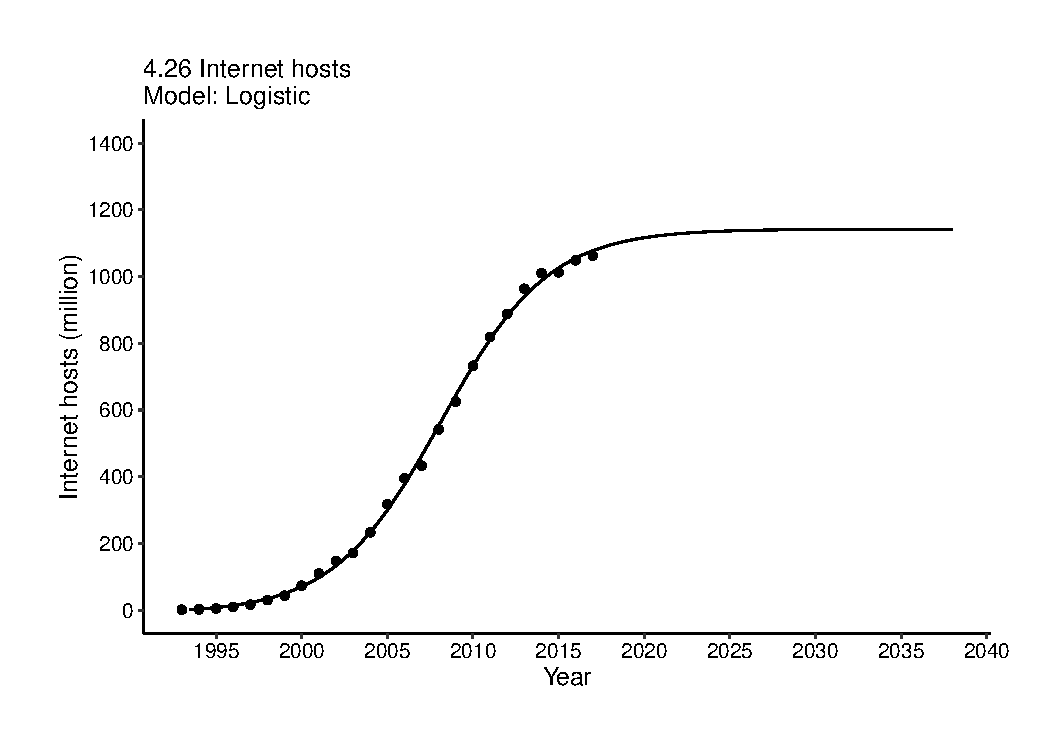
\includegraphics[width=8cm]{output/figs-ggplot/4.26.pdf}
\caption{\textbf{Dataset 4.26}: The post-1993 growth of Internet hosts has followed a logistic curve with the inflection year in 2008 and with the asymptotic value less than 10% above the 2017 total. Data from ISC (2017). }
\end{figure}
	
\begin{figure}[h]
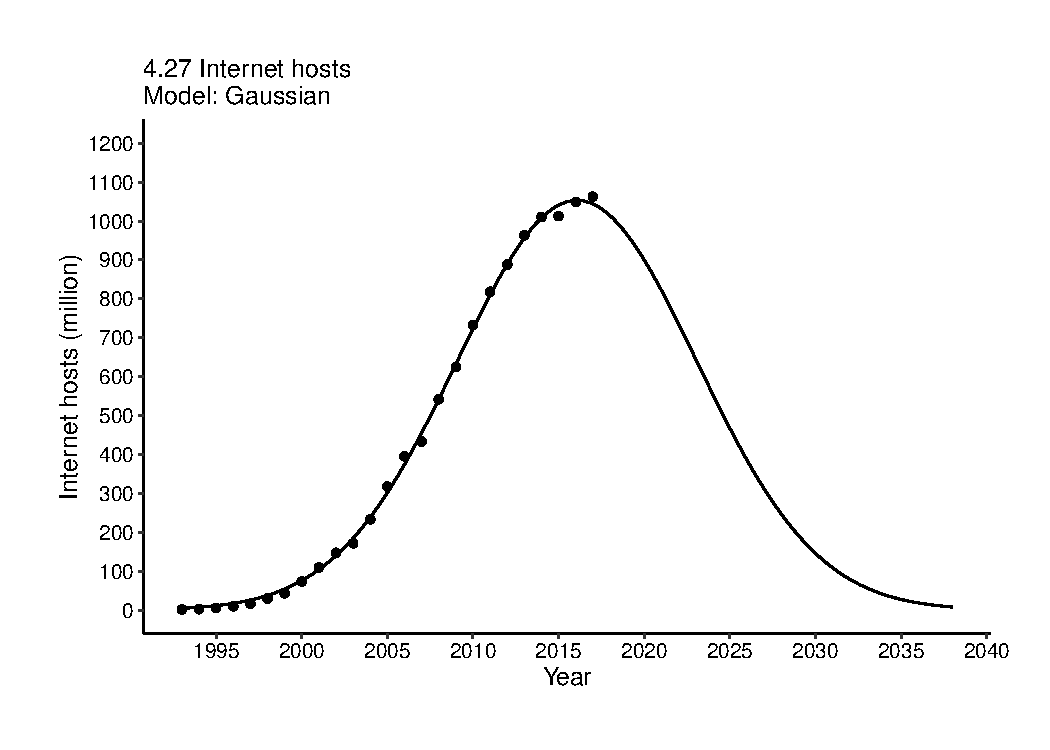
\includegraphics[width=8cm]{output/figs-ggplot/4.27.pdf}
\caption{\textbf{Dataset 4.27}: The growth of Internet hosts also fits a Gaussian curve peaking in 2016 and returning to negligible values before 2040. Such a development seems quite unlikely - unless a new mode of hosting takes over. Data from ISC (2017).}
\end{figure}
	
\begin{figure}[h]
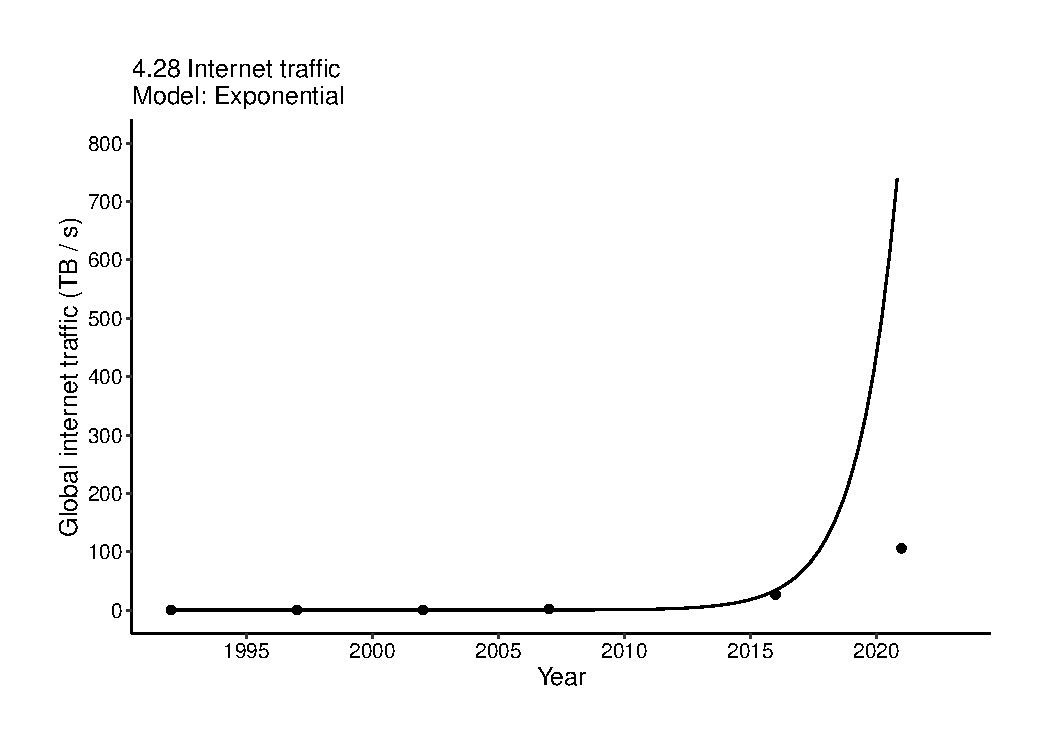
\includegraphics[width=8cm]{output/figs-ggplot/4.28.pdf}
\caption{\textbf{Dataset 4.28}: Post-1992 growth of Internet traffic in TB/s fits a logistic curve in its early stages of growth indicating further substantial gains in decades ahead. Data from CISCO (2017).}
\end{figure}
	
\begin{figure}[h]
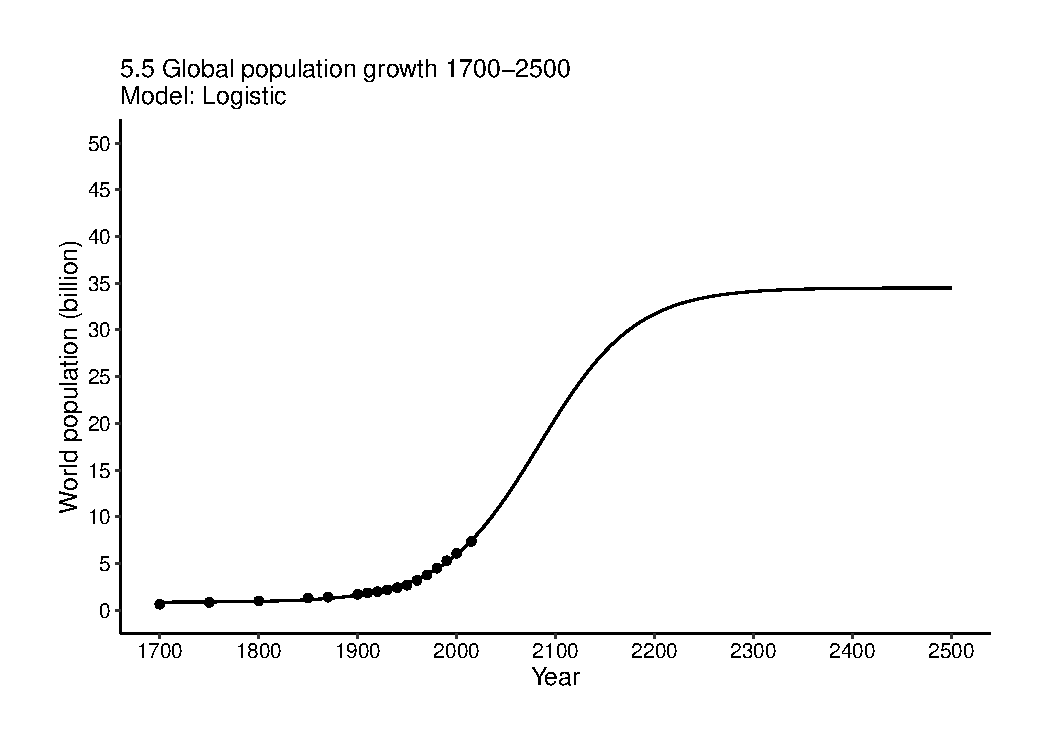
\includegraphics[width=8cm]{output/figs-ggplot/5.5.pdf}
\caption{\textbf{Dataset 5.5}: "Global population growth}
\end{figure}
	
\begin{figure}[h]
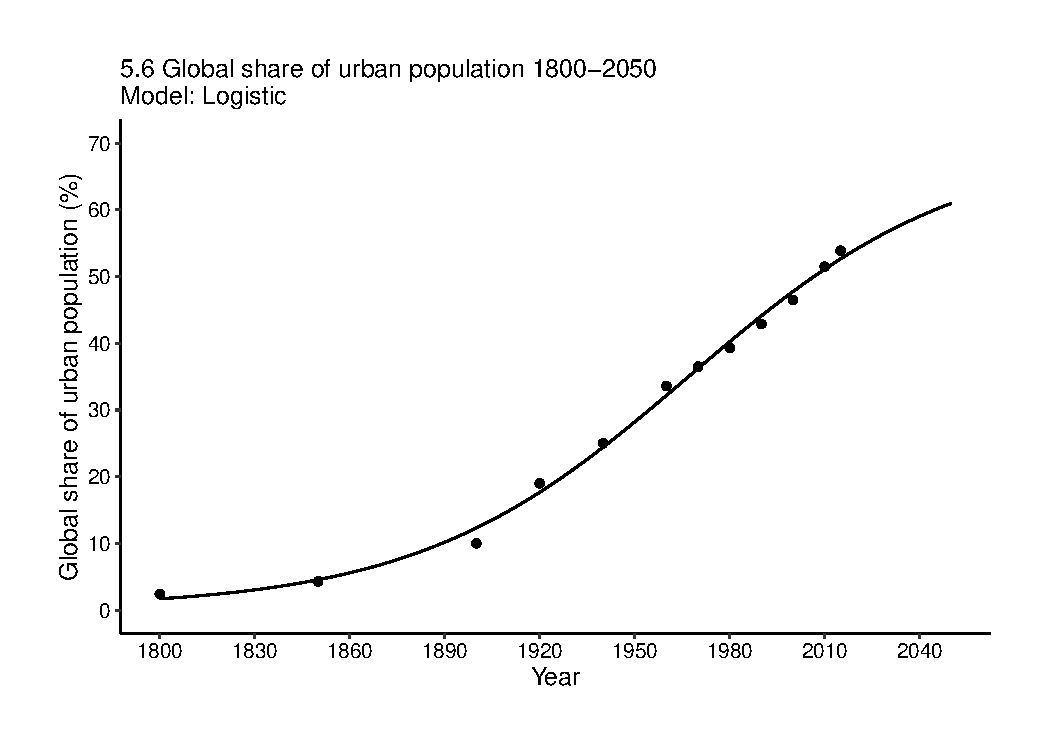
\includegraphics[width=8cm]{output/figs-ggplot/5.6.pdf}
\caption{\textbf{Dataset 5.6}: "Global share of the urban population}
\end{figure}
	
\begin{figure}[h]
\includegraphics[width=8cm]{output/figs-ggplot/5.7.pdf}
\caption{\textbf{Dataset 5.7}: "Share of the urban population in the US since 1790. Plotted from data in USBC (1975) and subsequent volumes of US Statistical Abstract. With the logistic curve inflected already in 1910}
\end{figure}
	
\begin{figure}[h]
\includegraphics[width=8cm]{output/figs-ggplot/5.9.pdf}
\caption{\textbf{Dataset 5.9}: Tokyo's population within prefectural boundaries (1900-2020) - a logistic curve with the inflection point in 1932 and asymptote at 13.8 million - and within the Tokyo Major Metropolitan Region since 1920: logistic curve infelction point in 1971 and asymptote at 38.8 million. Data from SB (1996) and TMG (2017). }
\end{figure}
	
\begin{figure}[h]
\includegraphics[width=8cm]{output/figs-ggplot/5.9.1.pdf}
\caption{\textbf{Dataset 5.9.1}: Tokyo's population within prefectural boundaries (1900-2020) - a logistic curve with the inflection point in 1932 and asymptote at 13.8 million - and within the Tokyo Major Metropolitan Region since 1920: logistic curve infelction point in 1971 and asymptote at 38.8 million. Data from SB (1996) and TMG (2017). }
\end{figure}
	
\begin{figure}[h]
\includegraphics[width=8cm]{output/figs-ggplot/5.9.2.pdf}
\caption{\textbf{Dataset 5.9.2}: Tokyo's population within prefectural boundaries (1900-2020) - a logistic curve with the inflection point in 1932 and asymptote at 13.8 million - and within the Tokyo Major Metropolitan Region since 1920: logistic curve infelction point in 1971 and asymptote at 38.8 million. Data from SB (1996) and TMG (2017). }
\end{figure}
	
\begin{figure}[h]
\includegraphics[width=8cm]{output/figs-ggplot/5.11.pdf}
\caption{\textbf{Dataset 5.11}: Logistic}
\end{figure}
	
\begin{figure}[h]
\includegraphics[width=8cm]{output/figs-ggplot/5.12.pdf}
\caption{\textbf{Dataset 5.12}: Gaussian}
\end{figure}
	
\begin{figure}[h]
\includegraphics[width=8cm]{output/figs-ggplot/5.13.pdf}
\caption{\textbf{Dataset 5.13}: Growth of global primary energy supply (including traditional biomass fuels) and fossil fuel and primary electricity supply since 1800. Data from Smil (2017b). }
\end{figure}
	
\begin{figure}[h]
\includegraphics[width=8cm]{output/figs-ggplot/5.13.1.pdf}
\caption{\textbf{Dataset 5.13.1}: Growth of global primary energy supply (including traditional biomass fuels) and fossil fuel and primary electricity supply since 1800. Data from Smil (2017b). }
\end{figure}
	
\begin{figure}[h]
\includegraphics[width=8cm]{output/figs-ggplot/5.13.2.pdf}
\caption{\textbf{Dataset 5.13.2}: Growth of global primary energy supply (including traditional biomass fuels) and fossil fuel and primary electricity supply since 1800. Data from Smil (2017b). }
\end{figure}
	
\begin{figure}[h]
\includegraphics[width=8cm]{output/figs-ggplot/5.14.pdf}
\caption{\textbf{Dataset 5.14}: Growth of global crude oil production since 1870. Data from Smil (2017b).}
\end{figure}
	
\begin{figure}[h]
\includegraphics[width=8cm]{output/figs-ggplot/5.15.pdf}
\caption{\textbf{Dataset 5.15}: Growth of global natural gas extraction since 1870. Data from Smil (2017b).}
\end{figure}
	
\begin{figure}[h]
\includegraphics[width=8cm]{output/figs-ggplot/5.16.pdf}
\caption{\textbf{Dataset 5.16}: "Growth of global coal produciton since 1800. While the two logistic curves for crude oil and natural gas provide a highly plausible indication of future development}
\end{figure}
	
\begin{figure}[h]
\includegraphics[width=8cm]{output/figs-ggplot/5.17.pdf}
\caption{\textbf{Dataset 5.17}: Growth of global electricity generation since 1900. Data from Smil (2017b) and BP (2017). }
\end{figure}
	
\begin{figure}[h]
\includegraphics[width=8cm]{output/figs-ggplot/5.18.pdf}
\caption{\textbf{Dataset 5.18}: Growth of global hydroelectricity generation since 1900. Data from Smil (2017b) and BP (2017).}
\end{figure}
	
\begin{figure}[h]
\includegraphics[width=8cm]{output/figs-ggplot/5.19.pdf}
\caption{\textbf{Dataset 5.19}: Growth of global nuclear generation since 1960. Data from Smil (2017b) and BP (2017).}
\end{figure}
	
\begin{figure}[h]
\includegraphics[width=8cm]{output/figs-ggplot/5.20.pdf}
\caption{\textbf{Dataset 5.20}: "Growth of global cropland}
\end{figure}
	
\begin{figure}[h]
\includegraphics[width=8cm]{output/figs-ggplot/5.21.pdf}
\caption{\textbf{Dataset 5.21}: "Growth of US cropland}
\end{figure}
	
\begin{figure}[h]
\includegraphics[width=8cm]{output/figs-ggplot/5.22.pdf}
\caption{\textbf{Dataset 5.22}: Growth of global grasslands. The inflection year was in 1923 and the total area is now less than 10% from the asymptotic level. Data from PBL (2010) and FAO (2018).}
\end{figure}
	
\begin{figure}[h]
\includegraphics[width=8cm]{output/figs-ggplot/5.23.pdf}
\caption{\textbf{Dataset 5.23}: Worldwide production of nitrogenous fertilizers since 1913. Another logistic curve that is very close to its asymptote. Data from Smil (2001) and FAO (2018).}
\end{figure}
	
\begin{figure}[h]
\includegraphics[width=8cm]{output/figs-ggplot/5.24.pdf}
\caption{\textbf{Dataset 5.24}: Global harvest of staple grain crops since 1900. Data from Smil (2013a) and FAO (2018).}
\end{figure}
	
\begin{figure}[h]
\includegraphics[width=8cm]{output/figs-ggplot/5.28.pdf}
\caption{\textbf{Dataset 5.28}: "Logistic curve of worldwide semiconductor sales}
\end{figure}
	
\begin{figure}[h]
\includegraphics[width=8cm]{output/figs-ggplot/5.29.pdf}
\caption{\textbf{Dataset 5.29}: "Growth and logistic outlook of GDBP (expression in international $2011) in four major economies - France}
\end{figure}
	
\begin{figure}[h]
\includegraphics[width=8cm]{output/figs-ggplot/5.29.1.pdf}
\caption{\textbf{Dataset 5.29.1}: "Growth and logistic outlook of GDBP (expression in international $2011) in four major economies - France}
\end{figure}
	
\begin{figure}[h]
\includegraphics[width=8cm]{output/figs-ggplot/5.29.2.pdf}
\caption{\textbf{Dataset 5.29.2}: "Growth and logistic outlook of GDBP (expression in international $2011) in four major economies - France}
\end{figure}
	
\begin{figure}[h]
\includegraphics[width=8cm]{output/figs-ggplot/5.29.3.pdf}
\caption{\textbf{Dataset 5.29.3}: "Growth and logistic outlook of GDBP (expression in international $2011) in four major economies - France}
\end{figure}
	
\begin{figure}[h]
\includegraphics[width=8cm]{output/figs-ggplot/5.29.4.pdf}
\caption{\textbf{Dataset 5.29.4}: "Growth and logistic outlook of GDBP (expression in international $2011) in four major economies - France}
\end{figure}
	
\begin{figure}[h]
\includegraphics[width=8cm]{output/figs-ggplot/5.30.pdf}
\caption{\textbf{Dataset 5.30}: "Growth of per capita income in the US}
\end{figure}
	
\begin{figure}[h]
\includegraphics[width=8cm]{output/figs-ggplot/5.30.1.pdf}
\caption{\textbf{Dataset 5.30.1}: "Growth of per capita income in the US}
\end{figure}
	
\begin{figure}[h]
\includegraphics[width=8cm]{output/figs-ggplot/5.30.2.pdf}
\caption{\textbf{Dataset 5.30.2}: "Growth of per capita income in the US}
\end{figure}
	
\begin{figure}[h]
\includegraphics[width=8cm]{output/figs-ggplot/5.30.3.pdf}
\caption{\textbf{Dataset 5.30.3}: "Growth of per capita income in the US}
\end{figure}
	
\begin{figure}[h]
\includegraphics[width=8cm]{output/figs-ggplot/5.31.pdf}
\caption{\textbf{Dataset 5.31}: Growing shares of international trade in the world economic product since 1870. Data from Klasing and Milionis (2014) and World Bank (2018).}
\end{figure}
	
\begin{figure}[h]
\includegraphics[width=8cm]{output/figs-ggplot/6.1.pdf}
\caption{\textbf{Dataset 6.1}: US crude oil extraction forecast based on the 1900-1980 trajectory. Data from USBC (1975) and USEIA (2019). }
\end{figure}
	
\begin{figure}[h]
\includegraphics[width=8cm]{output/figs-ggplot/6.2.pdf}
\caption{\textbf{Dataset 6.2}: Population of Greater London: best fits based on 1801-1981 (a) and 1801-2001 (b) totals. Data from Morrey (1978) and GLA (2015). }
\end{figure}
	
\begin{figure}[h]
\includegraphics[width=8cm]{output/figs-ggplot/6.2.1.pdf}
\caption{\textbf{Dataset 6.2.1}: Population of Greater London: best fits based on 1801-1981 (a) and 1801-2001 (b) totals. Data from Morrey (1978) and GLA (2015). }
\end{figure}
	
\begin{figure}[h]
\includegraphics[width=8cm]{output/figs-ggplot/6.2.2.pdf}
\caption{\textbf{Dataset 6.2.2}: Population of Greater London: best fits based on 1801-1981 (a) and 1801-2001 (b) totals. Data from Morrey (1978) and GLA (2015). }
\end{figure}
	
\begin{figure}[h]
\includegraphics[width=8cm]{output/figs-ggplot/6.7.pdf}
\caption{\textbf{Dataset 6.7}: "British steel output}
\end{figure}
	
\begin{figure}[h]
\includegraphics[width=8cm]{output/figs-ggplot/6.9.pdf}
\caption{\textbf{Dataset 6.9}: Number of American draft horses between 1850 and 1970 conforms closely to the normal curve trajectory. Data from USBC (1975). }
\end{figure}
	
\begin{figure}[h]
\includegraphics[width=8cm]{output/figs-ggplot/6.10.pdf}
\caption{\textbf{Dataset 6.10}: Number of US steam locomotives: a very good Gaussian fit for the nine decades between 1876 and 1967. Data from USBC (1975). }
\end{figure}
	
\begin{figure}[h]
\includegraphics[width=8cm]{output/figs-ggplot/6.11.pdf}
\caption{\textbf{Dataset 6.11}: The historical growth of the US passenger car fleet can be fitted quite well into a normal curve peaking around 2030. Data from USBC (1975) and from subsequent volumes of the US Statistical Abstract. }
\end{figure}
	
\end{document}
